% =============================================================================
% L09 (Class 9) --- textbook exercises with solutions. Built from the MPE list template
% (~/.claude/commands/templates/lista-exam.tex).
%
% TWO MODES (one source file):
%   \solucoesfalse  -> blank LIST (space to solve)
%   \solucoestrue   -> ANSWER KEY (same file)
%
% Compile (copyable PDF, global lmodern+cmap rule):
%   pdflatex lista-L09-book-exercises.tex  (run 2x) ; check: pdffonts ... (all Type 1)
% Numbers: python Listas/L09-book-exercises-check.py reproduces and asserts every number.
% =============================================================================
\documentclass[11pt,a4paper]{article}
\usepackage[utf8]{inputenc}
\usepackage[T1]{fontenc}
\usepackage{lmodern}   % Type 1 vector fonts (replaces PK bitmaps)
\usepackage{cmap}      % ToUnicode CMap -> copyable text and accents
\usepackage[english]{babel}
\usepackage{amsmath,amssymb,amsfonts,bm}
\usepackage[a4paper,margin=2.2cm]{geometry}
\usepackage{enumitem}
\usepackage{fancyhdr}
\usepackage{comment}
% One cut file per job: parallel builds in one folder would otherwise share comment.cut and
% swap solutions. Redefine DefaultCutFileName; overriding CommentCutFile alone is reset by comment.sty.
\def\DefaultCutFileName{\def\CommentCutFile{\jobname.cut}}
\usepackage{needspace}
\usepackage{xcolor}
\usepackage{microtype}
\usepackage{booktabs}
\usepackage{pgfplots}
\pgfplotsset{compat=1.17}

% ====================== CONFIGURATION ======================
\newif\ifsolucoes
\solucoesfalse                 % <<<< \solucoestrue for the ANSWER KEY; \solucoesfalse for the LIST

\newcommand{\disciplina}{Econometria Avançada --- MPE (Insper)}
\newcommand{\listatema}{L09 --- Multivariate time series (Class 9): textbook exercises}
\newcommand{\espacoresol}{4.5cm}   % height of the solving space in the blank list

% ====================== MACHINERY ======================
\ifsolucoes\includecomment{sol}\else\excludecomment{sol}\fi

\pagestyle{fancy}\fancyhf{}
\lhead{\footnotesize\disciplina}
\rhead{\footnotesize List L09\ifsolucoes{} --- Solutions\fi}
\cfoot{\footnotesize\thepage}
\renewcommand{\headrulewidth}{0.3pt}
\setlength{\headheight}{14pt}

\setlist{topsep=2pt,itemsep=2pt}
\newcounter{questao}
% Equations are numbered per question, (Q<question>.<n>), so they never collide with the
% books' own numbers, which keep their printed tags, e.g. (8.7) or (10.32).
\renewcommand{\theequation}{Q\thequestao.\arabic{equation}}

% Block header
\newcommand{\bloco}[3]{\bigskip\noindent
  {\large\bfseries\color{blue!55!black}Block #1 --- #2}\hfill\textit{(#3)}\par
  \noindent\rule{\linewidth}{0.3pt}\smallskip}

% Question (automatic numbering; resets the equation counter)
\newcommand{\questao}[1]{\refstepcounter{questao}\setcounter{equation}{0}\medskip\needspace{5\baselineskip}\noindent
  \textbf{Question \thequestao.}~#1\par}
% Source line that opens every question (estilo-avaliacao §5, book questions)
\newcommand{\fonte}[1]{\par\noindent{\small\textit{Source:} #1}\par\smallskip}

% Notation list that opens every solution (estilo-avaliacao §4, "Equations, notation and layout").
\newenvironment{notacao}{\par\smallskip\noindent\textbf{Notation.}\begin{itemize}[leftmargin=1.4em,topsep=1pt,itemsep=0pt]\small}{\end{itemize}}
\allowdisplaybreaks

% Solving space in the blank list
\newcommand{\resolespaco}{\ifsolucoes\else\par\textit{Solution:}\vspace{\espacoresol}\par\fi}

% Solution step (use inside sol)
\newcommand{\passo}[2]{\par\smallskip\noindent\textbf{Step --- #1.}~#2}
\newcommand{\intuicao}[1]{\par\smallskip\noindent\textit{Intuition.}~#1}
\newcommand{\refbib}[1]{\par\smallskip\noindent{\footnotesize\color{black!60}\textbf{Ref:} #1}}
% Code / output excerpts
\newenvironment{saida}{\par\smallskip\footnotesize\verbatim}{\endverbatim\par\smallskip}
\newcommand{\bx}{\bm{x}}\newcommand{\ba}{\bm{a}}\newcommand{\bb}{\bm{b}}\newcommand{\br}{\bm{r}}
\newcommand{\bmu}{\bm{\mu}}\newcommand{\bphi}{\bm{\phi}}\newcommand{\bSigma}{\bm{\Sigma}}
\newcommand{\bGamma}{\bm{\Gamma}}\newcommand{\bPhi}{\bm{\Phi}}\newcommand{\bI}{\bm{I}}

% =============================================================================
\begin{document}
\begin{center}
  {\Large\bfseries \disciplina}\\[2pt]
  {\large Exercise list: \listatema}\ifsolucoes\\[2pt]\textit{Solutions}\fi
\end{center}
\vspace{2pt}

{\footnotesize\noindent\textbf{Instructions.} These are the \emph{Practice} items of Class~9 in
\texttt{Map/class-plan.md}: Tsay 8.1, 8.2, 8.5, 8.7; Tsay 9.7; Tsay 10.1--10.6; Greenberg 10.4.
Every question opens with a source line, and the statement is reproduced verbatim from the book PDF.
Data exercises use Tsay's data files (\texttt{Listas/data/}, provenance in \texttt{Listas/data/README.md})
and are solved in Python (NumPy, SciPy, \texttt{statsmodels}); the multivariate GARCH models are
estimated by Gaussian maximum likelihood written in NumPy and \texttt{scipy.optimize}.
\texttt{Listas/L09-book-exercises-check.py} reproduces and asserts every number in the solutions.
Show your steps.\par}

% =============================================================================
\bloco{1}{Vector autoregressions, IRFs, forecasts and cointegration}{Tsay Ch.~8 \,\textbullet\, Questions 1--4}

% ---------------------------------------------------------------- Q1 = T 8.1
\questao{Cross-correlation matrices and the multivariate portmanteau test (Tsay 8.1).}
\fonte{Tsay (2010), \textit{Analysis of Financial Time Series}, 3rd ed., Chapter~8, Exercise~8.1,
printed p.~462. Reproduced verbatim.}

\begin{quote}\small
8.1. Consider the monthly log stock returns, in percentages and including dividends, of Merck \&
Company, Johnson \& Johnson, General Electric, General Motors, Ford Motor Company, and
value-weighted index from January 1960 to December 2008; see the file \texttt{m-mrk2vw.txt}.
\begin{enumerate}[label=(\alph*),leftmargin=2em]
\item Compute the sample mean, covariance matrix, and correlation matrix of the data.
\item Test the hypothesis $H_0:\bm{\rho}_1=\cdots=\bm{\rho}_6=\bm{0}$, where $\bm{\rho}_i$ is the lag-$i$
cross-correlation matrix of the data. Draw conclusions based on the 5\% significance level.
\item Is there any lead--lag relationship among the six return series?
\end{enumerate}
\end{quote}
\resolespaco
\begin{sol}
\begin{notacao}
\item $\br_t=(r_{1t},\dots,r_{6t})'$: monthly log returns (\%) of MRK, JNJ, GE, GM, F and the
value-weighted index VW, in this order; $t=1,\dots,T$, $T=588$ (Jan 1960--Dec 2008); $k=6$.
\item $\bar{\br}$: sample mean; $\hat{\bGamma}_\ell$: lag-$\ell$ sample cross-covariance matrix;
$\hat{\bm D}=\mathrm{diag}\{\hat\Gamma_{11}(0)^{1/2},\dots,\hat\Gamma_{kk}(0)^{1/2}\}$.
\item $\hat{\bm\rho}_\ell=[\hat\rho_{ij}(\ell)]$: lag-$\ell$ sample cross-correlation matrix;
$\rho_{ij}(\ell)=\mathrm{Corr}(r_{it},r_{j,t-\ell})$, so $\rho_{ij}(\ell)\neq0$ for $\ell>0$ means
$r_{jt}$ \emph{leads} $r_{it}$.
\item $Q_k(m)$: multivariate portmanteau statistic; $\chi^2_{\nu,0.95}$: 95\% quantile of a chi-squared with $\nu$ d.f.
\end{notacao}

\passo{(a) moments}{The estimators are Tsay's Eqs.~(8.5)--(8.6):
\begin{align}
\hat{\bGamma}_\ell&=\frac1T\sum_{t=\ell+1}^{T}(\br_t-\bar{\br})(\br_{t-\ell}-\bar{\br})',\label{eq:q1gam}\\
\hat{\bm\rho}_\ell&=\hat{\bm D}^{-1}\hat{\bGamma}_\ell\hat{\bm D}^{-1}.\label{eq:q1rho}
\end{align}
Applying them with $\ell=0$ (the covariance in the table uses the divisor $T-1$):}
\begin{center}\small
\begin{tabular}{lrrrrrr}
\toprule
 & MRK & JNJ & GE & GM & F & VW\\
\midrule
Mean & 0.967 & 1.170 & 0.721 & 0.124 & 0.449 & 0.725\\
\midrule
\multicolumn{7}{l}{Covariance matrix}\\
MRK & 49.58 & & & & & \\
JNJ & 23.87 & 39.59 & & & & \\
GE & 17.93 & 17.43 & 41.37 & & & \\
GM & 10.23 & 8.82 & 23.55 & 72.82 & & \\
F & 12.69 & 11.85 & 25.22 & 54.19 & 85.30 & \\
VW & 14.30 & 14.25 & 20.49 & 20.07 & 21.85 & 19.94\\
\midrule
\multicolumn{7}{l}{Correlation matrix}\\
JNJ & 0.539 & & & & & \\
GE & 0.396 & 0.431 & & & & \\
GM & 0.170 & 0.164 & 0.429 & & & \\
F & 0.195 & 0.204 & 0.425 & 0.688 & & \\
VW & 0.455 & 0.507 & 0.713 & 0.527 & 0.530 & \\
\bottomrule
\end{tabular}
\end{center}
All contemporaneous correlations are positive; the largest are GM--F (0.688, same industry) and
GE--VW (0.713, a large index constituent); the drug stocks are least correlated with the automakers.

\passo{(b) portmanteau test}{Tsay's Eq.~(8.7) is
\begin{equation}
Q_k(m)=T^2\sum_{\ell=1}^{m}\frac{1}{T-\ell}\,\mathrm{tr}\!\left(\hat{\bGamma}_\ell'\hat{\bGamma}_0^{-1}\hat{\bGamma}_\ell\hat{\bGamma}_0^{-1}\right)
\;\overset{H_0}{\sim}\;\chi^2_{k^2m}.\label{eq:q1Q}
\end{equation}
With $k=6$ and $m=6$, the degrees of freedom in \eqref{eq:q1Q} are
\begin{align}
k^2m&=(6)^2(6)\nonumber\\
&=216.\nonumber
\end{align}
Evaluating \eqref{eq:q1Q} with the matrices of \eqref{eq:q1gam}:
\begin{align}
Q_6(6)&=285.07,\qquad \chi^2_{216,0.95}=251.29,\qquad p=0.0011,\nonumber\\
Q_6(1)&=87.42,\qquad\ \ \chi^2_{36,0.95}=51.00,\qquad\ \ p=3.6\times10^{-6}.\nonumber
\end{align}
Since $285.07>251.29$, $H_0:\bm\rho_1=\cdots=\bm\rho_6=\bm0$ is rejected at 5\%: the six return
series have serial or cross dependence. The lag-1 matrix alone already rejects ($87.42>51.00$).}

\passo{(c) lead--lag}{Under $H_0$ each $\hat\rho_{ij}(\ell)$ is approximately $N(0,1/T)$, so the 5\% band is
\begin{align}
\frac{2}{\sqrt{T}}&=\frac{2}{\sqrt{588}}\nonumber\\
&=\frac{2}{24.249}\nonumber\\
&=0.0825.\nonumber
\end{align}
The entries of $\hat{\bm\rho}_1,\dots,\hat{\bm\rho}_6$ from \eqref{eq:q1rho} outside $\pm0.0825$ are:}
\begin{center}\small
\begin{tabular}{cllr}
\toprule
Lag $\ell$ & Row $i$ (today) & Column $j$ (lagged) & $\hat\rho_{ij}(\ell)$\\
\midrule
1 & GM & GE & 0.159\\
1 & GM & VW & 0.164\\
1 & F & VW & 0.104\\
1 & VW & VW & 0.100\\
3 & GE & JNJ & $-0.087$\\
3 & GM & MRK & 0.121\\
5 & GE & GM & 0.102\\
5 & VW & GM & 0.094\\
6 & VW & JNJ & $-0.086$\\
\bottomrule
\end{tabular}
\end{center}
The clearest pattern is at lag 1: last month's market return (VW) and GE return lead this month's
GM and Ford returns (0.164, 0.159, 0.104). With $6\cdot6\cdot6=216$ entries tested, about
$0.05\times216=10.8$ would exceed the band by chance alone, and only 9 do; so the isolated entries at
lags 3, 5 and 6 are weak evidence. Answer: there is a mild lead--lag relationship, the market and GE
leading the two automakers by one month; it is statistically detectable (the $Q$ test of part (b)),
but economically small ($|\hat\rho|<0.17$, i.e.\ under 3\% of variance).
\intuicao{A lead--lag correlation is a cross-correlation off the diagonal of $\bm\rho_\ell$ for
$\ell>0$. Slow diffusion of market-wide news into some stocks produces exactly this ``market leads
stock'' pattern; it is small for large, liquid stocks, as here.}
\refbib{Tsay (2010) \S8.1.1--8.1.4 (Eqs.~8.2--8.7), pp.~390--398.}
\end{sol}

% ---------------------------------------------------------------- Q2 = T 8.2
\questao{Bivariate AR and MA models for interest-rate changes; structural form (Tsay 8.2).}
\fonte{Tsay (2010), \textit{Analysis of Financial Time Series}, 3rd ed., Chapter~8, Exercise~8.2,
printed pp.~462--463. Reproduced verbatim.}

\begin{quote}\small
8.2. The Federal Reserve Bank of St.\ Louis publishes selected interest rates and U.S.\ financial data
on its website: \texttt{http://research.stlouisfed.org/fred2/}. Consider the monthly 1-year and
10-year Treasury constant maturity rates from April 1953 to October 2009 for 679 observations; see
the file \texttt{m-gs1n10.txt}. The rates are in percentages.
\begin{enumerate}[label=(\alph*),leftmargin=2em]
\item Let $c_t=r_t-r_{t-1}$ be the change series of the monthly interest rate $r_t$. Build a
bivariate autoregressive model for the two change series. Discuss the implications of the model.
Transform the model into a structural form.
\item Build a bivariate moving-average model for the two change series. Discuss the implications of
the model and compare it with the bivariate AR model built earlier.
\end{enumerate}
\end{quote}
\resolespaco
\begin{sol}
\begin{notacao}
\item $r_{1t}$, $r_{10,t}$: 1-year and 10-year rates (\%); $\bm c_t=(c_{1t},c_{2t})'$ with
$c_{1t}=r_{1t}-r_{1,t-1}$, $c_{2t}=r_{10,t}-r_{10,t-1}$; $T=678$ changes, $k=2$.
\item VAR($p$): $\bm c_t=\bphi_0+\sum_{i=1}^p\bPhi_i\bm c_{t-i}+\ba_t$, $\ba_t\sim(\bm0,\bSigma)$ white noise.
\item VMA($q$): $\bm c_t=\bm\theta_0+\ba_t-\sum_{j=1}^q\bm\Theta_j\ba_{t-j}$ (Tsay's sign convention, Eq.~8.23).
\item $\bSigma=\bm L\bm G\bm L'$: Cholesky factorisation, $\bm L$ unit lower triangular, $\bm G=\mathrm{diag}(g_{11},g_{22})$;
$\bb_t=\bm L^{-1}\ba_t$: orthogonal (structural) shocks.
\item $M(i)$: Tsay's sequential likelihood-ratio statistic for VAR($i$) vs VAR($i-1$), $\chi^2_{k^2}$ under $H_0$.
\end{notacao}

\passo{(a) order}{Tsay's Eq.~(8.18) is
\begin{equation}
M(i)=-\left(T-k-i-\tfrac32\right)\ln\frac{|\hat{\bSigma}_i|}{|\hat{\bSigma}_{i-1}|}\;\overset{H_0}{\sim}\;\chi^2_{4},\label{eq:q2M}
\end{equation}
with the 5\% critical value $\chi^2_{4,0.95}=9.49$. On a common sample (10 presample lags):}
\begin{center}\small
\begin{tabular}{lrrrrrrrr}
\toprule
$i$ & 1 & 2 & 3 & 4 & 5 & 6 & 7 & 8\\
\midrule
$M(i)$ & 135.33 & 57.25 & 13.38 & 8.10 & 4.44 & 43.09 & 0.87 & 10.15\\
\bottomrule
\end{tabular}
\end{center}
$M(6)=43.09$ is large and $M(7)=0.87$ is not; the Hannan--Quinn criterion also picks $p=6$ (AIC picks 8,
BIC picks 2). I use a VAR(6).

\passo{(a) fitted VAR(6)}{OLS on $t=7,\dots,678$ (672 equations per series) gives
$\hat\bphi_0=(-0.0025,\ 0.0006)'$ and (rows = equations for $c_{1t}$, $c_{2t}$; columns = lagged $c_1$, $c_2$):}
\begin{center}\scriptsize\setlength{\tabcolsep}{3pt}
\begin{tabular}{lrrrrrr}
\toprule
 & $\hat\bPhi_1$ & $\hat\bPhi_2$ & $\hat\bPhi_3$ & $\hat\bPhi_4$ & $\hat\bPhi_5$ & $\hat\bPhi_6$\\
\midrule
row 1 & $(0.324,\ 0.337)$ & $(-0.150,\ -0.234)$ & $(-0.032,\ 0.165)$ & $(-0.122,\ 0.006)$ & $(0.224,\ -0.047)$ & $(-0.314,\ 0.126)$\\
row 2 & $(-0.008,\ 0.434)$ & $(0.057,\ -0.320)$ & $(-0.123,\ 0.220)$ & $(0.000,\ -0.034)$ & $(0.161,\ -0.095)$ & $(-0.195,\ 0.113)$\\
\bottomrule
\end{tabular}
\end{center}
\begin{equation}
\hat{\bSigma}=\begin{pmatrix}0.1425&0.0723\\0.0723&0.0623\end{pmatrix},\qquad
\widehat{\mathrm{Corr}}(a_{1t},a_{2t})=0.768.\label{eq:q2Sig}
\end{equation}
Twelve of the 24 AR coefficients have $|t|>2$. The residual portmanteau is $Q_2(12)=55.65$ with
$k^2(12-6)=24$ d.f.\ ($p=0.0003$): some correlation is left, largely produced by the 1979--82
volatility burst, which a homoskedastic VAR cannot absorb.

\passo{(a) implications}{(i) The constants are essentially zero: neither rate has a drift, so the
levels behave like driftless I(1) series. (ii) The diagonal of $\hat\bPhi_1$ is positive (0.324,
0.434) and that of $\hat\bPhi_2$ negative: changes have short momentum followed by partial reversal.
(iii) Granger causality (Wald tests that the 6 cross coefficients are zero): the 10-year change
helps predict the 1-year change ($W=19.33$, 6 d.f., $p=0.0037$) and the 1-year change helps predict
the 10-year change ($W=46.38$, $p=10^{-7.6}$): there is feedback in both directions. (iv) The
contemporaneous correlation 0.768 in \eqref{eq:q2Sig} is far larger than any lagged effect: most
co-movement happens within the month.}

\passo{(a) structural form}{Write $\bSigma=\bm L\bm G\bm L'$ with
$\bm L=\begin{pmatrix}1&0\\ \ell_{21}&1\end{pmatrix}$. Equating elements,
\begin{align}
\ell_{21}&=\frac{\sigma_{21}}{\sigma_{11}},\label{eq:q2l}\\
g_{11}&=\sigma_{11},\qquad g_{22}=\sigma_{22}-\frac{\sigma_{21}^2}{\sigma_{11}}.\label{eq:q2g}
\end{align}
Substituting \eqref{eq:q2Sig} into \eqref{eq:q2l} and \eqref{eq:q2g}:
\begin{align}
\ell_{21}&=\frac{(0.0723)}{(0.1425)}=0.5075,\nonumber\\
g_{22}&=(0.0623)-\frac{(0.0723)^2}{(0.1425)}\nonumber\\
&=0.0623-0.03668\nonumber\\
&=0.0256,\qquad g_{11}=0.1425.\nonumber
\end{align}
Premultiplying the VAR by $\bm L^{-1}=\begin{pmatrix}1&0\\-\ell_{21}&1\end{pmatrix}$ (Tsay Eq.~8.9) gives
\begin{equation}
\bm L^{-1}\bm c_t=\bm L^{-1}\bphi_0+\sum_{i=1}^{6}\bm L^{-1}\bPhi_i\bm c_{t-i}+\bb_t,\qquad \mathrm{Cov}(\bb_t)=\bm G.\label{eq:q2str}
\end{equation}
Row 2 of $\bm L^{-1}\bPhi_i$ is (row 2 of $\bPhi_i$) $-\ell_{21}\times$(row 1 of $\bPhi_i$). For $i=1$, with
$\hat\bPhi_1=\begin{pmatrix}0.3243&0.3366\\-0.0085&0.4338\end{pmatrix}$:
\begin{align}
(-0.0085)-(0.5075)(0.3243)&=-0.0085-0.16458=-0.173,\nonumber\\
(0.4338)-(0.5075)(0.3366)&=0.4338-0.17082=0.263.\nonumber
\end{align}
The other lags follow the same way, and the constant is $0.0006-(0.5075)(-0.0025)=0.0019$. The
structural equation for the 10-year change, Tsay's Eq.~(8.10), is therefore
\begin{align}
c_{2t}={}&0.5075\,c_{1t}+0.0019-0.173c_{1,t-1}+0.263c_{2,t-1}+0.133c_{1,t-2}-0.201c_{2,t-2}\nonumber\\
&-0.106c_{1,t-3}+0.136c_{2,t-3}+0.062c_{1,t-4}-0.037c_{2,t-4}\nonumber\\
&+0.048c_{1,t-5}-0.071c_{2,t-5}-0.036c_{1,t-6}+0.050c_{2,t-6}+b_{2t},\nonumber
\end{align}
with $\mathrm{Var}(b_{2t})=0.0256$, while the first equation is the reduced-form equation for $c_{1t}$
($b_{1t}=a_{1t}$, $\mathrm{Var}=0.1425$). A 1-point surprise in the 1-year rate moves the 10-year rate by
about half a point in the same month; given $c_{1t}$, the residual variance of $c_{2t}$ drops from 0.0623 to 0.0256.}

\passo{(b) VMA}{The sample cross-correlation matrices of $\bm c_t$ are significant (beyond $2/\sqrt{678}=0.0768$) at
lags 1, 2, 3, 5, 6, 7, 9, 10 and 11, so they show no clean cut-off. I fit VMA($q$), $q=1,2,3$, by conditional maximum
likelihood ($\ba_0=\dots=\ba_{1-q}=\bm0$, Tsay \S8.3) and compare Tsay's criteria
$\mathrm{AIC}=\ln|\tilde{\bSigma}|+2k^2q/T$ and $\mathrm{BIC}=\ln|\tilde{\bSigma}|+k^2q\ln T/T$:}
\begin{center}\small
\begin{tabular}{lrrr}
\toprule
$q$ & 1 & 2 & 3\\
\midrule
AIC & $-5.5199$ & $-5.5365$ & $-5.5274$\\
BIC & $-5.4932$ & $-5.4831$ & $-5.4474$\\
\bottomrule
\end{tabular}
\end{center}
AIC selects $q=2$. The fitted VMA(2) (standard errors in parentheses) is
\begin{align}
\bm c_t=\begin{pmatrix}-0.0026\\0.0011\end{pmatrix}+\ba_t
-\begin{pmatrix}-0.324_{(0.061)}&-0.309_{(0.094)}\\ 0.013_{(0.040)}&-0.420_{(0.062)}\end{pmatrix}\ba_{t-1}
-\begin{pmatrix}0.083_{(0.069)}&-0.029_{(0.096)}\\ -0.028_{(0.041)}&0.131_{(0.058)}\end{pmatrix}\ba_{t-2},\nonumber
\end{align}
with $\tilde{\bSigma}=\begin{pmatrix}0.1507&0.0777\\0.0777&0.0657\end{pmatrix}$ (residual correlation 0.782).

\passo{(b) implications and comparison}{(i) The (2,1) elements of $\bm\Theta_1,\bm\Theta_2$ are
insignificant while $\Theta_{1,12}=-0.309$ is significant: past 10-year shocks feed into the 1-year
change, not the reverse, so the VMA suggests a one-way link, unlike the two-way Granger feedback of the
VAR. (ii) A VMA(2) implies zero cross-correlation beyond lag 2, which the data contradict: the residual
$Q_2(12)=111.14$ ($40$ d.f., $p=10^{-7.9}$) is twice the VAR(6) value of 55.65. (iii) AIC of the VAR(6)
computed the same way is $-5.5822<-5.5365$, so AIC prefers the VAR(6); BIC ($-5.4211$ for the VAR(6))
prefers the small VMA(1), but that model fails the residual check even more. The VAR(6) is the better
description; the VMA is useful only as a short-memory summary of the first two lags.}
\intuicao{AR and MA models are two parameterisations of the same linear dynamics. When the
cross-correlations decay slowly with bumps at several lags, a finite VMA needs many terms, while a VAR
captures the decay through its recursion.}
\refbib{Tsay (2010) \S8.2.1 (Eqs.~8.9--8.10), \S8.2.4 (Eqs.~8.16--8.19), \S8.3 (Eqs.~8.23--8.28), pp.~399--422.}
\end{sol}

% ---------------------------------------------------------------- Q3 = T 8.5
\questao{A seasonal bivariate AR(4) model (Tsay 8.5).}
\fonte{Tsay (2010), \textit{Analysis of Financial Time Series}, 3rd ed., Chapter~8, Exercise~8.5,
printed p.~463. Reproduced verbatim.}

\begin{quote}\small
8.5. The bivariate AR(4) model $\bx_t-\bPhi_4\bx_{t-4}=\bphi_0+\ba_t$ is a special seasonal model with
periodicity 4, where $\{\ba_t\}$ is a sequence of independent and identically distributed normal
random vectors with mean zero and covariance matrix $\bSigma$. Such a seasonal model may be useful in
studying quarterly earnings of a company. (a) Assume that $\bx_t$ is weakly stationary. Derive the
mean vector and covariance matrix of $\bx_t$. (b) Derive the necessary and sufficient condition of weak
stationarity for $\bx_t$. (c) Show that $\bGamma_\ell=\bPhi_4\bGamma_{\ell-4}$ for $\ell>0$, where
$\bGamma_\ell$ is the lag-$\ell$ autocovariance matrix of $\bx_t$.
\end{quote}
\resolespaco
\begin{sol}
\begin{notacao}
\item $\bx_t$: $2\times1$ observed vector; $\bphi_0$: $2\times1$ constant; $\bPhi_4$: $2\times2$ seasonal
coefficient matrix with eigenvalues $\lambda_1,\lambda_2$ (possibly complex).
\item $\ba_t\overset{iid}{\sim}N(\bm0,\bSigma)$, $\bSigma$ positive definite; $\ba_t$ independent of $\bx_{t-j}$, $j\geq1$.
\item $\bmu=E(\bx_t)$; $\tilde\bx_t=\bx_t-\bmu$; $\bGamma_\ell=E(\tilde\bx_t\tilde\bx_{t-\ell}')$, with $\bGamma_{-\ell}=\bGamma_\ell'$ (Tsay Eq.~8.2).
\item $B$: back-shift operator, $B\bx_t=\bx_{t-1}$; $\otimes$: Kronecker product; $\mathrm{vec}$: column stacking.
\end{notacao}
The model is
\begin{equation}
\bx_t=\bphi_0+\bPhi_4\bx_{t-4}+\ba_t.\label{eq:q3m}
\end{equation}

\passo{(a) mean}{Take expectations of \eqref{eq:q3m}; weak stationarity gives $E(\bx_t)=E(\bx_{t-4})=\bmu$:
\begin{align}
\bmu&=\bphi_0+\bPhi_4\bmu+\bm0,\nonumber\\
(\bI-\bPhi_4)\bmu&=\bphi_0,\nonumber\\
\bmu&=(\bI-\bPhi_4)^{-1}\bphi_0.\label{eq:q3mu}
\end{align}
The inverse exists because, under the condition of part (b), 1 is not an eigenvalue of $\bPhi_4$.}

\passo{(a) covariance}{From \eqref{eq:q3mu}, $\bphi_0=(\bI-\bPhi_4)\bmu$. Substituting into \eqref{eq:q3m}:
\begin{align}
\bx_t&=\left((\bI-\bPhi_4)\bmu\right)+\bPhi_4\bx_{t-4}+\ba_t,\nonumber\\
\tilde\bx_t&=\bPhi_4\tilde\bx_{t-4}+\ba_t.\label{eq:q3dev}
\end{align}
Multiply \eqref{eq:q3dev} by its own transpose and take expectations; the cross terms vanish because
$\ba_t$ is independent of $\tilde\bx_{t-4}$, and $E(\tilde\bx_{t-4}\tilde\bx_{t-4}')=\bGamma_0$:
\begin{align}
\bGamma_0&=E\!\left[(\bPhi_4\tilde\bx_{t-4}+\ba_t)(\bPhi_4\tilde\bx_{t-4}+\ba_t)'\right]\nonumber\\
&=\bPhi_4\bGamma_0\bPhi_4'+\bSigma.\label{eq:q3G0}
\end{align}
Apply $\mathrm{vec}(\bm A\bm X\bm B)=(\bm B'\otimes\bm A)\mathrm{vec}(\bm X)$ to \eqref{eq:q3G0}:
\begin{align}
\mathrm{vec}(\bGamma_0)&=(\bPhi_4\otimes\bPhi_4)\mathrm{vec}(\bGamma_0)+\mathrm{vec}(\bSigma),\nonumber\\
\mathrm{vec}(\bGamma_0)&=(\bI_4-\bPhi_4\otimes\bPhi_4)^{-1}\mathrm{vec}(\bSigma).\label{eq:q3vec}
\end{align}
Equivalently, substituting \eqref{eq:q3dev} into itself repeatedly gives
\begin{equation*}
\tilde\bx_t=\sum_{j\ge0}\bPhi_4^j\ba_{t-4j},\qquad\text{hence}\qquad \bGamma_0=\sum_{j\ge0}\bPhi_4^j\bSigma(\bPhi_4')^j.
\end{equation*}}

\passo{(b) stationarity}{Write \eqref{eq:q3dev} as $(\bI-\bPhi_4B^4)\tilde\bx_t=\ba_t$. The process is weakly
stationary if and only if every zero of $\det(\bI-\bPhi_4z^4)$ lies outside the unit circle. Put $w=z^4$:
\begin{align}
\det(\bI-\bPhi_4w)&=(1-\lambda_1w)(1-\lambda_2w),\label{eq:q3det}
\end{align}
whose zeros are $w_i=1/\lambda_i$. Each $w_i$ gives four values of $z$ with
\begin{align}
|z|&=|w_i|^{1/4}\nonumber\\
&=|\lambda_i|^{-1/4}.\nonumber
\end{align}
So $|z|>1$ for every zero if and only if $|\lambda_i|<1$, $i=1,2$. The same follows from the companion
form (Tsay Eq.~8.15): with $\bPhi_1=\bPhi_2=\bPhi_3=\bm0$, the $8\times8$ companion matrix $\bm F$ has
$\det(\bm F-\nu\bI_8)=\det(\nu^4\bI_2-\bPhi_4)$, so its eigenvalues solve $\nu^4=\lambda_i$, and
$|\nu|<1\iff|\lambda_i|<1$. \textbf{Condition:} all eigenvalues of $\bPhi_4$ have modulus less than one;
for a $2\times2$ matrix this is $|\det\bPhi_4|<1$ and $|\mathrm{tr}\,\bPhi_4|<1+\det\bPhi_4$.}

\passo{(c) autocovariances}{For $\ell>0$, postmultiply \eqref{eq:q3dev} by $\tilde\bx_{t-\ell}'$ and take expectations:
\begin{align}
E(\tilde\bx_t\tilde\bx_{t-\ell}')&=\bPhi_4E(\tilde\bx_{t-4}\tilde\bx_{t-\ell}')+E(\ba_t\tilde\bx_{t-\ell}').\label{eq:q3post}
\end{align}
$\tilde\bx_{t-\ell}$ depends only on $\ba_{t-\ell},\ba_{t-\ell-4},\dots$, all dated before $t$, so
$E(\ba_t\tilde\bx_{t-\ell}')=\bm0$. By stationarity the first expectation on the right depends only on the
lag between $t-4$ and $t-\ell$, which is $\ell-4$: $E(\tilde\bx_{t-4}\tilde\bx_{t-\ell}')=\bGamma_{\ell-4}$
(for $\ell<4$ this is $\bGamma_{4-\ell}'$). Substituting both into \eqref{eq:q3post}:
\begin{align}
\bGamma_\ell&=\bPhi_4\left(\bGamma_{\ell-4}\right)+\left(\bm0\right)\nonumber\\
&=\bPhi_4\bGamma_{\ell-4},\qquad \ell>0.\label{eq:q3c}
\end{align}
A consequence: by \eqref{eq:q3c}, $\bGamma_{4m}=\bPhi_4^m\bGamma_0$, while $\bGamma_1=\bPhi_4\bGamma_3'$ and
$\bGamma_3=\bPhi_4\bGamma_1'$ give $\bGamma_1=\bPhi_4\bGamma_1\bPhi_4'$, so
$(\bI_4-\bPhi_4\otimes\bPhi_4)\mathrm{vec}(\bGamma_1)=\bm0$ and $\bGamma_1=\bGamma_3=\bm0$; similarly
$\bGamma_2=\bPhi_4\bGamma_2\bPhi_4'$ gives $\bGamma_2=\bm0$. Only lags that are multiples of 4 are correlated.}
\intuicao{The model links each quarter only to the same quarter one year earlier, so the series is four
interleaved VAR(1) processes in $\bPhi_4$ that never talk to each other: correlation appears only at
seasonal lags and decays geometrically as $\bPhi_4^m$. The check script verifies \eqref{eq:q3vec},
the companion eigenvalues and \eqref{eq:q3c} numerically on a simulated example.}
\refbib{Tsay (2010) \S8.2.2--8.2.3 (Eqs.~8.11--8.15), pp.~401--405.}
\end{sol}

% ---------------------------------------------------------------- Q4 = T 8.7
\questao{VAR, impulse responses, forecasts, cointegration and ECM for 1- and 3-year rates (Tsay 8.7).}
\fonte{Tsay (2010), \textit{Analysis of Financial Time Series}, 3rd ed., Chapter~8, Exercise~8.7,
printed pp.~463--464. Reproduced verbatim.}

\begin{quote}\small
8.7. Consider the monthly U.S.\ 1-year and 3-year Treasury constant maturity rates from April 1953 to
March 2004. The data can be obtained from the Federal Reserve Bank of St.\ Louis or from the file
\texttt{m-gs1n3-5304.txt} (1-year, 3-year, dates). See also Example 8.6, which uses a shorter data span.
Here we use the interest rates directly without the log transformation and define
$\bx_t=(x_{1t},x_{2t})'$, where $x_{1t}$ is the 1-year maturity rate and $x_{2t}$ is the 3-year maturity rate.
\begin{enumerate}[label=(\alph*),leftmargin=2em]
\item Identify a VAR model for the bivariate interest rate series. Write down the fitted model.
\item Compute the impulse response functions of the fitted VAR model. It suffices to use the first 6 lags.
\item Use the fitted VAR model to produce 1-step- to 12-step-ahead forecasts of the interest rates,
assuming that the forecast origin is March 2004.
\item Are the two interest rate series cointegrated, when a restricted constant term is used? Use 5\%
significance level to perform the test.
\item If the series are cointegrated, build an ECM for the series. Write down the fitted model.
\item Use the fitted ECM to produce 1-step- to 12-step-ahead forecasts of the interest rates, assuming
that the forecast origin is March 2004.
\item Compare the forecasts produced by the VAR model and the ECM.
\end{enumerate}
\end{quote}
\resolespaco
\begin{sol}
\begin{notacao}
\item $\bx_t=(x_{1t},x_{2t})'$: 1-year and 3-year rates (\%), Apr 1953--Mar 2004, $T=612$; origin
$h=T$ (March 2004) with $\bx_T=(1.19,\ 2.00)'$.
\item VAR($p$) as in Q2; $\bm\Psi_i$: MA (impulse-response) matrices, $\bx_t=\bmu+\sum_{i\ge0}\bm\Psi_i\ba_{t-i}$, $\bm\Psi_0=\bI$.
\item $\bm P$: lower-triangular Cholesky factor, $\bm P\bm P'=\bSigma$ (equals $\bm L\bm G^{1/2}$ of Q2);
$\bm\Psi_i\bm P$: responses to one-standard-deviation orthogonal shocks.
\item $\hat\bx_T(\ell)$: $\ell$-step forecast; ECM: $\Delta\bx_t=\bm\alpha(\bm\beta'\bx_{t-1}+c_0)+\sum_{i=1}^{p-1}\bm\Gamma_i^*\Delta\bx_{t-i}+\ba_t$.
\item $\hat\lambda_1>\hat\lambda_2$: squared partial canonical correlations; $\mathrm{LR}_{tr}(m)$, $\mathrm{LR}_{max}(m)$: Johansen statistics.
\end{notacao}

\passo{(a) identification}{BIC over $p=1,\dots,12$ (common sample) is $-5.599$, $-5.756$, $-5.788$,
$-5.776$, $-5.744$ for $p=1,\dots,5$ and rises afterwards, so BIC selects $p=3$ (HQ picks 7 and AIC 12).
I adopt the VAR(3), as Tsay does with BIC for the T-bill rates of \S8.6.5. OLS gives
\begin{align}
\bx_t={}&\begin{pmatrix}0.0586\\0.0744\end{pmatrix}
+\begin{pmatrix}1.160&0.357\\0.018&1.405\end{pmatrix}\bx_{t-1}
+\begin{pmatrix}-0.287&-0.507\\0.014&-0.700\end{pmatrix}\bx_{t-2}
+\begin{pmatrix}0.108&0.158\\0.006&0.248\end{pmatrix}\bx_{t-3}+\ba_t,\label{eq:q4var}\\
\hat{\bSigma}={}&\begin{pmatrix}0.16573&0.12922\\0.12922&0.11669\end{pmatrix}.\label{eq:q4sig}
\end{align}
Standard errors of $\hat\bPhi_1$ are $(0.110,\ 0.130;\ 0.092,\ 0.109)$. The largest companion
eigenvalue modulus is $0.9856$: the fitted VAR is stationary but very close to a unit root. The residual
$Q_2(12)=151.36$ (36 d.f.) rejects whiteness for this and every $p\le11$, because the residuals have strong
volatility clustering (1979--82); I keep the parsimonious BIC choice.}

\passo{(b) impulse responses}{From $(\bI-\bPhi_1B-\bPhi_2B^2-\bPhi_3B^3)(\bI+\bm\Psi_1B+\cdots)=\bI$ (Tsay Eq.~8.21),
\begin{equation}
\bm\Psi_i=\sum_{j=1}^{\min(i,3)}\bPhi_j\bm\Psi_{i-j},\qquad \bm\Psi_0=\bI.\label{eq:q4psi}
\end{equation}
For $i=1$, \eqref{eq:q4psi} gives $\bm\Psi_1=\bPhi_1$. For the orthogonal responses, the Cholesky factor of
\eqref{eq:q4sig} is
\begin{align}
P_{11}&=\sqrt{0.16573}=0.40710,\nonumber\\
P_{21}&=\frac{(0.12922)}{(0.40710)}=0.31742,\nonumber\\
P_{22}&=\sqrt{(0.11669)-(0.31742)^2}=\sqrt{0.11669-0.100756}=\sqrt{0.015934}=0.1262.\nonumber
\end{align}
The responses (rows: $\ell$; entries $(i,j)$ = response of $x_{i,t+\ell}$ to shock $j$ at $t$) are:}
\begin{center}\small
\begin{tabular}{c|rrrr|rrrr}
\toprule
 & \multicolumn{4}{c|}{$\bm\Psi_\ell$ (to $\ba_t$)} & \multicolumn{4}{c}{$\bm\Psi_\ell\bm P$ (to 1-s.d.\ orthogonal $\bb_t$)}\\
$\ell$ & (1,1) & (1,2) & (2,1) & (2,2) & (1,1) & (1,2) & (2,1) & (2,2)\\
\midrule
0 & 1 & 0 & 0 & 1 & 0.407 & 0 & 0.317 & 0.126\\
1 & 1.160 & 0.357 & 0.018 & 1.405 & 0.586 & 0.045 & 0.453 & 0.177\\
2 & 1.066 & 0.410 & 0.061 & 1.280 & 0.564 & 0.052 & 0.431 & 0.162\\
3 & 1.024 & 0.276 & 0.115 & 1.075 & 0.504 & 0.035 & 0.388 & 0.136\\
4 & 1.020 & 0.198 & 0.164 & 0.974 & 0.478 & 0.025 & 0.376 & 0.123\\
5 & 1.014 & 0.200 & 0.204 & 0.943 & 0.476 & 0.025 & 0.382 & 0.119\\
6 & 1.002 & 0.217 & 0.239 & 0.916 & 0.477 & 0.027 & 0.388 & 0.116\\
\bottomrule
\end{tabular}
\end{center}
A one-standard-deviation shock to the 1-year rate (0.41 points) raises the 1-year rate by 0.59 one month
later and still by 0.48 after six months, and carries the 3-year rate up by 0.32--0.45: shocks are
almost permanent, as the near-unit eigenvalue implies. The orthogonal 3-year shock (0.13 points) has
small effects on the 1-year rate. With the ordering $(x_1,x_2)$ the 1-year shock is allowed to move the
3-year rate on impact but not vice versa (Tsay \S8.2.5 warns that the orthogonal IRF depends on the ordering).

\passo{(c) VAR forecasts}{Iterating \eqref{eq:q4var} with $\ba_{T+j}$ replaced by $\bm0$ from the last three
observations gives (forecast standard errors at $\ell=1,6,12$: $(0.407,0.342)$, $(1.242,1.025)$, $(1.681,1.418)$):}
\begin{center}\small
\begin{tabular}{c|rrrrrrrrrrrr}
\toprule
$\ell$ & 1 & 2 & 3 & 4 & 5 & 6 & 7 & 8 & 9 & 10 & 11 & 12\\
\midrule
VAR $x_1$ & 1.149 & 1.210 & 1.308 & 1.386 & 1.442 & 1.495 & 1.552 & 1.611 & 1.668 & 1.725 & 1.780 & 1.835\\
VAR $x_2$ & 1.917 & 1.969 & 2.039 & 2.082 & 2.110 & 2.139 & 2.173 & 2.210 & 2.247 & 2.284 & 2.321 & 2.359\\
ECM $x_1$ & 1.110 & 1.113 & 1.153 & 1.175 & 1.178 & 1.179 & 1.183 & 1.190 & 1.196 & 1.200 & 1.205 & 1.209\\
ECM $x_2$ & 1.884 & 1.890 & 1.912 & 1.911 & 1.896 & 1.881 & 1.871 & 1.863 & 1.856 & 1.848 & 1.841 & 1.834\\
\bottomrule
\end{tabular}
\end{center}
(The ECM rows are derived in part (f).)

\passo{(d) cointegration test}{With a restricted constant (Tsay's case 2, $\bmu_t=\bm\alpha c_0$), the
Johansen test uses Eqs.~(8.40)--(8.42) with the constant moved inside the error-correction term, VAR order
$p=3$ and $T-p=609$. The eigenvalues are $\hat\lambda_1=0.043548$, $\hat\lambda_2=0.006076$, with
$-\ln(1-\hat\lambda_1)=0.044524$ and $-\ln(1-\hat\lambda_2)=0.006094$. Tsay's Eq.~(8.42) is
\begin{equation}
\mathrm{LR}_{tr}(m)=-(T-p)\sum_{i=m+1}^{k}\ln(1-\hat\lambda_i).\label{eq:q4tr}
\end{equation}
Substituting into \eqref{eq:q4tr}:
\begin{align}
\mathrm{LR}_{tr}(0)&=(609)\left[(0.044524)+(0.006094)\right]=(609)(0.050618)=30.83,\nonumber\\
\mathrm{LR}_{tr}(1)&=(609)(0.006094)=3.71,\nonumber\\
\mathrm{LR}_{max}(0)&=(609)(0.044524)=27.12.\nonumber
\end{align}
The 5\% critical values for a restricted constant with $k=2$ (printed by Tsay, p.~439) are 19.96 and
9.24 for the trace test and 15.67 and 9.24 for the maximum-eigenvalue test. Since $30.83>19.96$
(and $27.12>15.67$) we reject $H(0)$; since $3.71<9.24$ we do not reject $H(1)$. \textbf{The two rates are
cointegrated with one cointegrating vector.}}

\passo{(e) ECM}{Maximum likelihood with rank 1 (normalised $\beta_1=1$) gives
$\hat{\bm\beta}=(1,\ -1.00875)'$ and $\hat c_0=0.47503$, so the stationary spread is
\begin{equation}
w_t=x_{1t}-1.00875\,x_{2t}+0.47503,\label{eq:q4w}
\end{equation}
and the fitted ECM (standard errors of $\bm\alpha$ in parentheses) is
\begin{align}
\Delta\bx_t={}&\begin{pmatrix}-0.0276_{(0.0329)}\\0.0313_{(0.0276)}\end{pmatrix}w_{t-1}
+\begin{pmatrix}0.190&0.336\\-0.012&0.442\end{pmatrix}\Delta\bx_{t-1}
+\begin{pmatrix}-0.098&-0.175\\0.002&-0.262\end{pmatrix}\Delta\bx_{t-2}+\ba_t,\nonumber\\
\hat{\bSigma}={}&\begin{pmatrix}0.1648&0.1285\\0.1285&0.1160\end{pmatrix}.\nonumber
\end{align}
The signs are those of error correction: when $w_{t-1}>0$ (1-year rate high relative to the 3-year rate)
$x_1$ falls and $x_2$ rises. Individually the loadings are imprecise, but the speed at which $w_t$
itself corrects is $\hat{\bm\beta}'\hat{\bm\alpha}=(-0.0276)+(-1.00875)(0.0313)=-0.0592$ per month, a
half-life of $\ln 0.5/\ln(1-0.0592)\approx11.4$ months. The checked Johansen eigenvector of part (d)
reproduces $(1,-1.00875,0.47503)$.}

\passo{(f) ECM forecasts}{Iterate the ECM for $\Delta\bx_{T+\ell}$ and cumulate from $\bx_T$; at the
origin, by \eqref{eq:q4w},
\begin{align}
w_T&=(1.19)-1.00875(2.00)+0.47503\nonumber\\
&=1.19-2.01750+0.47503\nonumber\\
&=-0.3525.\nonumber
\end{align}
The forecasts are the ECM rows of the table in part (c).}

\passo{(g) comparison}{(i) The VAR forecasts climb steadily (to 1.84 and 2.36 after a year) because the
levels VAR, though nearly integrated, is stationary and reverts to its implied mean
$(\bI-\hat\bPhi_1-\hat\bPhi_2-\hat\bPhi_3)^{-1}\hat\bphi_0=(5.671,\ 6.093)'$, the 1953--2004 average
level. (ii) The ECM imposes one unit root with no drift (restricted constant), so its forecasts stay near
the March 2004 levels (1.21 and 1.83 after a year); the only systematic movement closes the spread:
$w_T=-0.35<0$ means the 3-year rate is high relative to the 1-year rate, so the ECM forecasts a slightly
rising 1-year rate and a falling 3-year rate. (iii) The two sets differ by up to about 0.6 points at
$\ell=12$, inside the forecast standard errors (about 1.7 and 1.4 for the VAR). Which is better depends on
whether rates are believed to revert to a long-run mean; the ECM respects the unit-root and
cointegration evidence of part (d) and does not rely on the weak mean reversion of a nearly integrated VAR.}
\intuicao{Cointegration says the two rates share one stochastic trend: their spread is stationary even
though each rate wanders. A VAR in levels estimates this only implicitly and lets the near-unit root
pull forecasts towards the sample mean; the ECM writes the restriction down.}
\refbib{Tsay (2010) \S8.2.4--8.2.6 (Eqs.~8.16--8.22), \S8.5--8.6 (Eqs.~8.33--8.42), pp.~405--445.}
\end{sol}

% =============================================================================
\bloco{2}{Factor models}{Tsay Ch.~9 \,\textbullet\, Question 5}

% ---------------------------------------------------------------- Q5 = T 9.7
\questao{A macroeconomic factor model with VAR surprises (Tsay 9.7).}
\fonte{Tsay (2010), \textit{Analysis of Financial Time Series}, 3rd ed., Chapter~9, Exercise~9.7,
printed p.~503. Reproduced verbatim.}

\begin{quote}\small
9.7. The file \texttt{m-fedip.txt} contains year, month, effective federal funds rate, and the
industrial production index from July 1954 to December 2003. The industrial production index is
seasonally adjusted. Use the federal funds rate and the industrial production index as the
macroeconomic variables. Fit a macroeconomic factor model to the 10 excess returns in
\texttt{m-excess-c10sp-9003.txt}. You can use a VAR model to obtain the surprise series of the
macroeconomic variables. Comment on the fitted factor model.
\end{quote}
\resolespaco
\begin{sol}
\begin{notacao}
\item $FF_t$: effective federal funds rate (\%); $IP_t$: industrial production index; Jul 1954--Dec 2003 (594 months).
\item $\bm z_t=(\Delta FF_t,\ 100\,\Delta\ln IP_t)'$: change in the funds rate (points) and IP growth (\%), Aug 1954--Dec 2003.
\item $\bm f_t=(f_{1t},f_{2t})'$: surprises = residuals of a VAR for $\bm z_t$; $\bm\Sigma_f$: their covariance.
\item $r_{it}$: excess return (\%) of stock $i=1,\dots,10$ (ABT, LLY, MRK, PFE, F, GM, BP, CVX, RD, XOM), Jan 1990--Dec 2003, $T=168$.
\item $\alpha_i$, $\bm\beta_i=(\beta_{i1},\beta_{i2})$: intercept and loadings; $\epsilon_{it}$: specific factor, variance $\sigma_i^2$.
\end{notacao}

\passo{surprises}{The funds rate is highly persistent, so I model its monthly change, and IP through its
growth rate, as Tsay does for CPI and employment in \S9.2.2. BIC over VAR orders $0,\dots,12$ selects
$p=2$; the surprises are the VAR(2) residuals
\begin{equation}
\bm f_t=\bm z_t-\hat\bphi_0-\hat\bPhi_1\bm z_{t-1}-\hat\bPhi_2\bm z_{t-2},\qquad
\hat{\bm\Sigma}_f=\begin{pmatrix}0.2603&0.0741\\0.0741&0.6660\end{pmatrix},\label{eq:q5f}
\end{equation}
of which the last 168 (Jan 1990--Dec 2003) enter the factor model. A longer sample is used for the VAR so that
the surprises are not fitted on the return period alone.}

\passo{factor model}{Tsay's Eq.~(9.4) stacks the model $r_{it}=\alpha_i+\bm\beta_i\bm f_t+\epsilon_{it}$ as
\begin{equation}
\bm R=\bm G\bm\xi+\bm E,\qquad \bm G=[\bm 1_T,\ \bm F],\quad \bm\xi=[\bm\alpha,\ \bm\beta]',\label{eq:q5mlr}
\end{equation}
estimated by least squares, with residual variances and $R^2$ (Tsay \S9.2):
\begin{align}
\hat{\bm\xi}&=(\bm G'\bm G)^{-1}\bm G'\bm R,\label{eq:q5xi}\\
\hat\sigma_i^2&=\frac{[\hat{\bm E}'\hat{\bm E}]_{ii}}{T-m-1},\qquad m=2,\label{eq:q5s2}\\
R_i^2&=1-\frac{[\hat{\bm E}'\hat{\bm E}]_{ii}}{[\tilde{\bm R}'\tilde{\bm R}]_{ii}},\label{eq:q5r2}
\end{align}
where $\tilde{\bm R}$ is the mean-corrected return matrix. Applying \eqref{eq:q5xi}--\eqref{eq:q5r2} with the
surprises \eqref{eq:q5f} ($t$ ratios in parentheses):}
\begin{center}\footnotesize\setlength{\tabcolsep}{4pt}
\begin{tabular}{lrrrrrrrrrr}
\toprule
 & ABT & LLY & MRK & PFE & F & GM & BP & CVX & RD & XOM\\
\midrule
$\hat\beta_{FF}$ & $-2.52$ & $-2.42$ & $-0.50$ & $-4.93$ & $-13.34$ & $-7.77$ & $-4.91$ & $-3.84$ & $-4.22$ & $-3.25$\\
 & $(-0.83)$ & $(-0.57)$ & $(-0.13)$ & $(-1.34)$ & $(-2.85)$ & $(-1.72)$ & $(-1.60)$ & $(-1.40)$ & $(-1.46)$ & $(-1.53)$\\
$\hat\beta_{IP}$ & $-1.06$ & $-0.06$ & $-2.37$ & $-1.77$ & $1.64$ & $1.50$ & $-0.50$ & $-0.35$ & $-1.81$ & $-0.94$\\
 & $(-1.08)$ & $(-0.04)$ & $(-1.95)$ & $(-1.49)$ & $(1.08)$ & $(1.03)$ & $(-0.51)$ & $(-0.39)$ & $(-1.93)$ & $(-1.37)$\\
$\hat\sigma_i$ & 6.20 & 8.73 & 7.66 & 7.52 & 9.58 & 9.24 & 6.28 & 5.60 & 5.93 & 4.34\\
$R^2_i$ & 0.013 & 0.002 & 0.023 & 0.027 & 0.050 & 0.021 & 0.018 & 0.014 & 0.039 & 0.028\\
\bottomrule
\end{tabular}
\end{center}

\passo{comments}{(i) Every loading on the funds-rate surprise is negative: an unexpected tightening
lowers excess returns, most for the cyclical automakers (Ford $-13.34$, GM $-7.77$). Only Ford's is
significant at 5\% ($t=-2.85$). (ii) IP surprises have mixed signs and none is significant: positive for
the automakers, negative for drugs and oil. (iii) The fit is very poor: $R^2$ ranges from 0.002 to 0.050.
(iv) The implied covariance $\hat{\bm\beta}\hat{\bm\Sigma}_f\hat{\bm\beta}'+\hat{\bm D}$ gives correlations of
at most 0.032 between stocks, while the sample correlations average 0.308; the residual correlations
(average 0.302, largest 0.736 between CVX and RD) are almost the raw ones, so the specific factors are
far from uncorrelated and the diagonal $\bm D$ assumption fails. Macro surprises in the funds rate and
output explain little of these stocks' co-movement, which is driven by market and industry factors (the
BARRA and statistical factor models of Exercises 9.4--9.6).}
\intuicao{Prices react to news, so only the unexpected part of a macro variable should move returns; a
VAR removes the predictable part. Monthly macro surprises are, however, small and noisy relative to
stock-specific and industry news, which is why such models typically have tiny $R^2$, as Tsay also
finds with CPI and employment surprises (\S9.2.2).}
\refbib{Tsay (2010) \S9.1--9.2 (Eqs.~9.1--9.4), pp.~468--476.}
\end{sol}

% =============================================================================
\bloco{3}{Multivariate volatility models}{Tsay Ch.~10 \,\textbullet\, Questions 6--11}

{\small\noindent\textbf{Common setup for Questions 6--11.} Returns are converted to log returns in
percent, $r_{it}=100\ln(1+R_{it})$. All models are estimated by Gaussian maximum likelihood, the
log density of a shock $\ba_t$ being $-\tfrac12[k\ln2\pi+\ln|\bSigma_t|+\ba_t'\bSigma_t^{-1}\ba_t]$; the
recursions start at the sample covariance; standard errors come from the inverse numerical Hessian.
Adequacy uses the multivariate Ljung--Box statistic $Q_k(m)$ of Tsay's Eq.~(8.7) applied to the
standardized residuals $\tilde\ba_t=\bSigma_t^{-1/2}\ba_t$ (symmetric square root) and to $\tilde\ba_t^2$,
with $k^2m$ degrees of freedom (Tsay p.~533). Figures plot every sixth month.\par}

% ---------------------------------------------------------------- Q6 = T 10.1
\questao{EWMA covariance matrix for IBM, HPQ and the S\&P index (Tsay 10.1).}
\fonte{Tsay (2010), \textit{Analysis of Financial Time Series}, 3rd ed., Chapter~10, Exercise~10.1,
printed p.~554. Reproduced verbatim.}

\begin{quote}\small
10.1. Consider the monthly simple returns, including dividends, of IBM stock, Hewlett-Packard (HPQ)
stock, and the S\&P composite index from January 1962 to December 2008 for 564 observations. The returns
are in the file \texttt{m-ibmhpqsp6208.txt}. Transform into log returns in percentages. Use the
exponentially weighted moving-average method to obtain a multivariate volatility series for the three
return series. What is the estimated $\lambda$? Plot the three volatility series.
\end{quote}
\resolespaco
\begin{sol}
\begin{notacao}
\item $\br_t=(r_{1t},r_{2t},r_{3t})'$: log returns (\%) of IBM, HPQ, S\&P; $T=564$; $\bmu$: mean vector; $\ba_t=\br_t-\bmu$.
\item $\bSigma_t=\mathrm{Cov}(\ba_t\mid F_{t-1})$; $\lambda\in(0,1)$: EWMA smoothing parameter;
$\sigma_{ii,t}^{1/2}$: volatility of asset $i$.
\end{notacao}

\passo{model}{For large $t$, Tsay's Eq.~(10.2) reduces to the recursion
\begin{equation}
\bSigma_t=(1-\lambda)\ba_{t-1}\ba_{t-1}'+\lambda\bSigma_{t-1},\label{eq:q6ewma}
\end{equation}
and $(\bmu,\lambda)$ are estimated jointly by maximizing
\begin{equation}
\ln L(\bmu,\lambda)=-\frac12\sum_{t=1}^{T}\left[3\ln2\pi+\ln|\bSigma_t|+\ba_t'\bSigma_t^{-1}\ba_t\right],\label{eq:q6ll}
\end{equation}
with $\bSigma_t$ from \eqref{eq:q6ewma} (Tsay p.~507). Descriptive statistics: means $(0.622,\ 0.955,\
0.450)$, standard deviations $(7.157,\ 9.716,\ 4.341)$; the univariate $Q(12)$ of the returns are 7.08,
7.12 and 11.40, so a constant mean is enough.}

\passo{estimate}{Maximizing \eqref{eq:q6ll} gives $\hat\bmu=(0.631,\ 0.906,\ 0.397)'$ and
\begin{equation}
\hat\lambda=0.9687\ (\text{s.e. }0.0065),\qquad \ln L=-5316.80.\label{eq:q6lam}
\end{equation}
So each month the newest cross-product $\ba_{t-1}\ba_{t-1}'$ gets weight $1-\hat\lambda=0.0313$, and
by \eqref{eq:q6ewma} a shock's weight halves after
\begin{align}
\frac{\ln0.5}{\ln\hat\lambda}&=\frac{-0.693147}{\ln(0.96872)}\nonumber\\
&=\frac{-0.693147}{-0.031781}\nonumber\\
&=21.8\ \text{months}.\nonumber
\end{align}
This is a smoother filter than Tsay's daily example ($\hat\lambda=0.9305$), as expected for monthly data.}

\passo{volatility series}{The fitted volatilities $\hat\sigma_{ii,t}^{1/2}$ range over $[4.79,\ 12.18]$ for IBM,
$[7.44,\ 15.20]$ for HPQ and $[2.92,\ 6.31]$ for the S\&P index:}
\begin{center}
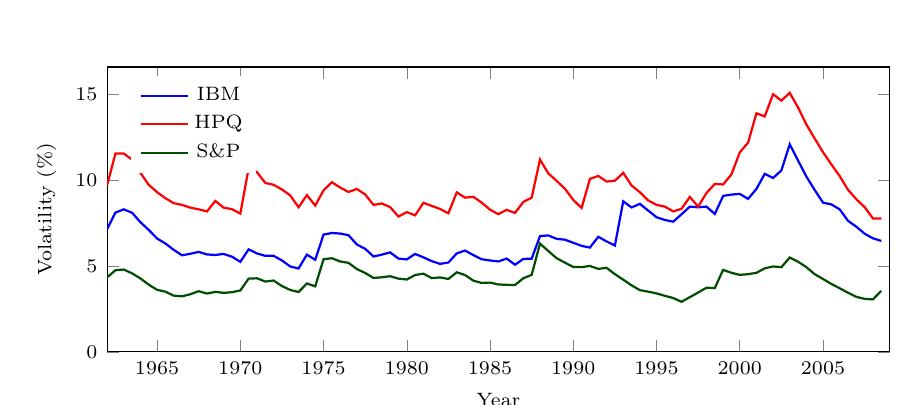
\begin{tikzpicture}
\begin{axis}[width=0.95\linewidth,height=5.2cm,xmin=1962,xmax=2009,ymin=0,
  xlabel={Year},ylabel={Volatility (\%)},legend pos=north west,legend style={font=\scriptsize,draw=none},
  tick label style={font=\scriptsize,/pgf/number format/1000 sep={}},label style={font=\scriptsize}]
\addplot[blue,thick] coordinates {(1962.00,7.16) (1962.50,8.12) (1963.00,8.31) (1963.50,8.11) (1964.00,7.56) (1964.50,7.11) (1965.00,6.61) (1965.50,6.32) (1966.00,5.95) (1966.50,5.63) (1967.00,5.72) (1967.50,5.83) (1968.00,5.68) (1968.50,5.65) (1969.00,5.71) (1969.50,5.55) (1970.00,5.25) (1970.50,5.98) (1971.00,5.74) (1971.50,5.60) (1972.00,5.60) (1972.50,5.33) (1973.00,4.98) (1973.50,4.86) (1974.00,5.67) (1974.50,5.37) (1975.00,6.84) (1975.50,6.93) (1976.00,6.90) (1976.50,6.80) (1977.00,6.26) (1977.50,6.01) (1978.00,5.56) (1978.50,5.67) (1979.00,5.80) (1979.50,5.44) (1980.00,5.39) (1980.50,5.71) (1981.00,5.51) (1981.50,5.29) (1982.00,5.13) (1982.50,5.21) (1983.00,5.74) (1983.50,5.91) (1984.00,5.64) (1984.50,5.40) (1985.00,5.33) (1985.50,5.27) (1986.00,5.44) (1986.50,5.08) (1987.00,5.42) (1987.50,5.43) (1988.00,6.75) (1988.50,6.79) (1989.00,6.59) (1989.50,6.54) (1990.00,6.36) (1990.50,6.18) (1991.00,6.08) (1991.50,6.71) (1992.00,6.44) (1992.50,6.20) (1993.00,8.78) (1993.50,8.42) (1994.00,8.63) (1994.50,8.24) (1995.00,7.85) (1995.50,7.69) (1996.00,7.59) (1996.50,8.02) (1997.00,8.47) (1997.50,8.43) (1998.00,8.47) (1998.50,8.04) (1999.00,9.09) (1999.50,9.17) (2000.00,9.21) (2000.50,8.92) (2001.00,9.50) (2001.50,10.38) (2002.00,10.14) (2002.50,10.58) (2003.00,12.10) (2003.50,11.16) (2004.00,10.22) (2004.50,9.44) (2005.00,8.70) (2005.50,8.60) (2006.00,8.31) (2006.50,7.64) (2007.00,7.30) (2007.50,6.89) (2008.00,6.62) (2008.50,6.47)};
\addlegendentry{IBM}
\addplot[red,thick] coordinates {(1962.00,9.72) (1962.50,11.56) (1963.00,11.56) (1963.50,11.21) (1964.00,10.44) (1964.50,9.74) (1965.00,9.31) (1965.50,8.96) (1966.00,8.67) (1966.50,8.57) (1967.00,8.41) (1967.50,8.31) (1968.00,8.19) (1968.50,8.80) (1969.00,8.41) (1969.50,8.32) (1970.00,8.06) (1970.50,10.70) (1971.00,10.48) (1971.50,9.85) (1972.00,9.74) (1972.50,9.47) (1973.00,9.12) (1973.50,8.43) (1974.00,9.14) (1974.50,8.53) (1975.00,9.42) (1975.50,9.89) (1976.00,9.58) (1976.50,9.32) (1977.00,9.50) (1977.50,9.18) (1978.00,8.57) (1978.50,8.65) (1979.00,8.44) (1979.50,7.89) (1980.00,8.15) (1980.50,7.96) (1981.00,8.69) (1981.50,8.51) (1982.00,8.33) (1982.50,8.08) (1983.00,9.30) (1983.50,8.99) (1984.00,9.04) (1984.50,8.70) (1985.00,8.29) (1985.50,8.03) (1986.00,8.28) (1986.50,8.10) (1987.00,8.74) (1987.50,8.99) (1988.00,11.21) (1988.50,10.41) (1989.00,9.97) (1989.50,9.51) (1990.00,8.86) (1990.50,8.39) (1991.00,10.08) (1991.50,10.26) (1992.00,9.93) (1992.50,9.98) (1993.00,10.44) (1993.50,9.70) (1994.00,9.31) (1994.50,8.83) (1995.00,8.57) (1995.50,8.47) (1996.00,8.19) (1996.50,8.34) (1997.00,9.03) (1997.50,8.47) (1998.00,9.26) (1998.50,9.79) (1999.00,9.76) (1999.50,10.35) (2000.00,11.63) (2000.50,12.20) (2001.00,13.91) (2001.50,13.73) (2002.00,15.02) (2002.50,14.65) (2003.00,15.10) (2003.50,14.25) (2004.00,13.26) (2004.50,12.44) (2005.00,11.64) (2005.50,10.93) (2006.00,10.25) (2006.50,9.45) (2007.00,8.90) (2007.50,8.44) (2008.00,7.78) (2008.50,7.77)};
\addlegendentry{HPQ}
\addplot[black!70!green,thick] coordinates {(1962.00,4.34) (1962.50,4.76) (1963.00,4.80) (1963.50,4.58) (1964.00,4.28) (1964.50,3.92) (1965.00,3.62) (1965.50,3.51) (1966.00,3.28) (1966.50,3.24) (1967.00,3.36) (1967.50,3.54) (1968.00,3.40) (1968.50,3.50) (1969.00,3.44) (1969.50,3.48) (1970.00,3.58) (1970.50,4.27) (1971.00,4.29) (1971.50,4.10) (1972.00,4.16) (1972.50,3.84) (1973.00,3.61) (1973.50,3.49) (1974.00,3.99) (1974.50,3.82) (1975.00,5.40) (1975.50,5.46) (1976.00,5.27) (1976.50,5.19) (1977.00,4.83) (1977.50,4.60) (1978.00,4.31) (1978.50,4.35) (1979.00,4.41) (1979.50,4.27) (1980.00,4.22) (1980.50,4.48) (1981.00,4.56) (1981.50,4.30) (1982.00,4.34) (1982.50,4.25) (1983.00,4.64) (1983.50,4.48) (1984.00,4.15) (1984.50,4.02) (1985.00,4.04) (1985.50,3.93) (1986.00,3.91) (1986.50,3.90) (1987.00,4.29) (1987.50,4.49) (1988.00,6.31) (1988.50,5.88) (1989.00,5.46) (1989.50,5.20) (1990.00,4.95) (1990.50,4.94) (1991.00,5.01) (1991.50,4.84) (1992.00,4.90) (1992.50,4.53) (1993.00,4.21) (1993.50,3.88) (1994.00,3.60) (1994.50,3.51) (1995.00,3.41) (1995.50,3.27) (1996.00,3.14) (1996.50,2.92) (1997.00,3.19) (1997.50,3.46) (1998.00,3.74) (1998.50,3.72) (1999.00,4.78) (1999.50,4.61) (2000.00,4.49) (2000.50,4.53) (2001.00,4.61) (2001.50,4.87) (2002.00,4.98) (2002.50,4.94) (2003.00,5.50) (2003.50,5.26) (2004.00,4.94) (2004.50,4.53) (2005.00,4.25) (2005.50,3.96) (2006.00,3.71) (2006.50,3.45) (2007.00,3.21) (2007.50,3.09) (2008.00,3.06) (2008.50,3.56)};
\addlegendentry{S\&P}
\end{axis}
\end{tikzpicture}
\end{center}
HPQ is always the most volatile and the index the least (diversification). All three rise after the
October 1987 crash and in 2000--2003 (the technology bust, strongest for HPQ); IBM's volatility jumps in
1993 (its restructuring crisis). Because $\hat\lambda$ is close to one, the series move slowly.
\intuicao{EWMA is a GARCH(1,1) without a constant and with $\alpha+\beta=1$ imposed on every element of
$\bSigma_t$ through a single $\lambda$: cheap, always positive definite, but it has no mean reversion,
so its forecasts are flat.}
\refbib{Tsay (2010) \S10.1 (Eq.~10.2, Example 10.1), pp.~506--510.}
\end{sol}

% ---------------------------------------------------------------- Q7 = T 10.2
\questao{DVEC(1,1) model for IBM and HPQ (Tsay 10.2).}
\fonte{Tsay (2010), \textit{Analysis of Financial Time Series}, 3rd ed., Chapter~10, Exercise~10.2,
printed p.~554. Reproduced verbatim.}

\begin{quote}\small
10.2. Focus on the monthly log returns of IBM and HPQ stocks from January 1962 to December 2008. Fit a
DVEC(1,1) model to the bivariate return series. Is the model adequate? Plot the fitted volatility series
and the time-varying correlations.
\end{quote}
\resolespaco
\begin{sol}
\begin{notacao}
\item $\br_t=(r_{1t},r_{2t})'$: IBM and HPQ log returns (\%), $T=564$; $\ba_t=\br_t-\bmu$; $\bSigma_t=[\sigma_{ij,t}]$.
\item $\bm A_0,\bm A_1,\bm B_1$: symmetric $2\times2$ parameter matrices; $\odot$: element-by-element product.
\item $\rho_{21,t}=\sigma_{21,t}/(\sigma_{11,t}\sigma_{22,t})^{1/2}$: conditional correlation.
\end{notacao}

\passo{model}{Tsay's Eq.~(10.5) with $m=s=1$ is
\begin{equation}
\bSigma_t=\bm A_0+\bm A_1\odot(\ba_{t-1}\ba_{t-1}')+\bm B_1\odot\bSigma_{t-1},\label{eq:q7dvec}
\end{equation}
i.e.\ each element follows its own GARCH(1,1)-type equation,
$\sigma_{ij,t}=A_{ij,0}+A_{ij,1}a_{i,t-1}a_{j,t-1}+B_{ij,1}\sigma_{ij,t-1}$.}

\passo{estimates}{Maximum likelihood (11 parameters, $\ln L=-3873.45$) gives
$\hat\mu_1=0.703_{(0.284)}$, $\hat\mu_2=1.124_{(0.386)}$, and
\begin{align}
\sigma_{11,t}&=2.998_{(1.616)}+0.065_{(0.025)}\,a_{1,t-1}^2+0.874_{(0.053)}\,\sigma_{11,t-1},\nonumber\\
\sigma_{21,t}&=4.283_{(2.344)}+0.066_{(0.024)}\,a_{1,t-1}a_{2,t-1}+0.802_{(0.086)}\,\sigma_{21,t-1},\nonumber\\
\sigma_{22,t}&=6.158_{(2.566)}+0.071_{(0.021)}\,a_{2,t-1}^2+0.864_{(0.040)}\,\sigma_{22,t-1}.\nonumber
\end{align}
All ARCH and GARCH coefficients are significant; the persistence $A_{ii,1}+B_{ii,1}$ is
$0.065+0.874=0.939$ and $0.071+0.864=0.935$ for the variances, a little lower for the covariance.
$\hat\bSigma_t$ is positive definite at every $t$ (checked), although \eqref{eq:q7dvec} does not guarantee it.}

\passo{adequacy}{For the standardized residuals:}
\begin{center}\small
\begin{tabular}{lrrrr}
\toprule
 & $Q_2(5)$ & $Q_2(10)$ & $Q_2^{(2)}(5)$ (squares) & $Q_2^{(2)}(10)$ (squares)\\
\midrule
Statistic & 18.54 & 31.91 & 29.97 & 45.19\\
$p$ value ($\chi^2_{20}$, $\chi^2_{40}$) & 0.552 & 0.815 & 0.070 & 0.264\\
\bottomrule
\end{tabular}
\end{center}
The univariate Ljung--Box $Q(12)$ of the squared standardized residuals have $p$ values 0.987 (IBM) and
0.248 (HPQ). No statistic rejects at 5\%: \textbf{the DVEC(1,1) model is adequate} for the first two
conditional moments.

\passo{plots}{The fitted volatilities and correlation:}
\begin{center}
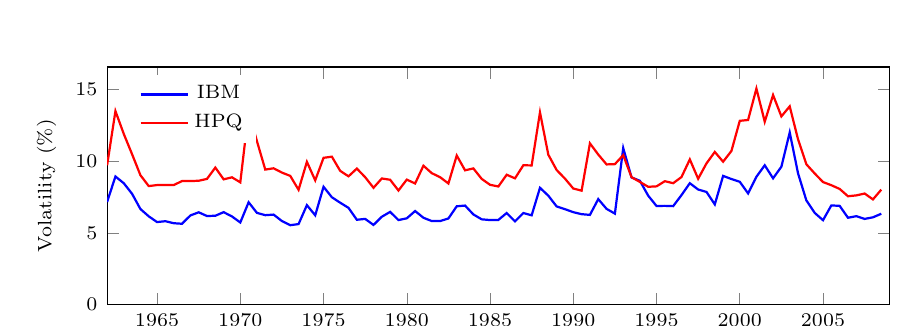
\begin{tikzpicture}
\begin{axis}[width=0.95\linewidth,height=4.6cm,xmin=1962,xmax=2009,ymin=0,
  ylabel={Volatility (\%)},legend pos=north west,legend style={font=\scriptsize,draw=none},
  tick label style={font=\scriptsize,/pgf/number format/1000 sep={}},label style={font=\scriptsize}]
\addplot[blue,thick] coordinates {(1962.00,7.16) (1962.50,8.94) (1963.00,8.47) (1963.50,7.73) (1964.00,6.67) (1964.50,6.16) (1965.00,5.76) (1965.50,5.82) (1966.00,5.68) (1966.50,5.64) (1967.00,6.22) (1967.50,6.44) (1968.00,6.18) (1968.50,6.20) (1969.00,6.45) (1969.50,6.15) (1970.00,5.73) (1970.50,7.14) (1971.00,6.40) (1971.50,6.24) (1972.00,6.28) (1972.50,5.83) (1973.00,5.54) (1973.50,5.62) (1974.00,6.94) (1974.50,6.23) (1975.00,8.22) (1975.50,7.49) (1976.00,7.11) (1976.50,6.75) (1977.00,5.92) (1977.50,5.98) (1978.00,5.56) (1978.50,6.13) (1979.00,6.47) (1979.50,5.90) (1980.00,6.02) (1980.50,6.53) (1981.00,6.06) (1981.50,5.83) (1982.00,5.83) (1982.50,6.01) (1983.00,6.86) (1983.50,6.91) (1984.00,6.29) (1984.50,5.95) (1985.00,5.90) (1985.50,5.91) (1986.00,6.39) (1986.50,5.81) (1987.00,6.39) (1987.50,6.23) (1988.00,8.15) (1988.50,7.60) (1989.00,6.85) (1989.50,6.66) (1990.00,6.45) (1990.50,6.31) (1991.00,6.26) (1991.50,7.36) (1992.00,6.68) (1992.50,6.35) (1993.00,10.92) (1993.50,8.87) (1994.00,8.64) (1994.50,7.60) (1995.00,6.88) (1995.50,6.89) (1996.00,6.87) (1996.50,7.64) (1997.00,8.47) (1997.50,8.03) (1998.00,7.86) (1998.50,6.99) (1999.00,8.98) (1999.50,8.76) (2000.00,8.57) (2000.50,7.76) (2001.00,8.92) (2001.50,9.72) (2002.00,8.81) (2002.50,9.62) (2003.00,12.01) (2003.50,9.16) (2004.00,7.27) (2004.50,6.40) (2005.00,5.89) (2005.50,6.92) (2006.00,6.89) (2006.50,6.06) (2007.00,6.17) (2007.50,5.98) (2008.00,6.09) (2008.50,6.34)};
\addlegendentry{IBM}
\addplot[red,thick] coordinates {(1962.00,9.72) (1962.50,13.50) (1963.00,11.91) (1963.50,10.49) (1964.00,9.03) (1964.50,8.27) (1965.00,8.34) (1965.50,8.34) (1966.00,8.34) (1966.50,8.62) (1967.00,8.62) (1967.50,8.64) (1968.00,8.77) (1968.50,9.56) (1969.00,8.74) (1969.50,8.88) (1970.00,8.53) (1970.50,13.49) (1971.00,11.40) (1971.50,9.42) (1972.00,9.51) (1972.50,9.21) (1973.00,8.98) (1973.50,8.01) (1974.00,9.96) (1974.50,8.67) (1975.00,10.24) (1975.50,10.32) (1976.00,9.33) (1976.50,8.95) (1977.00,9.49) (1977.50,8.89) (1978.00,8.15) (1978.50,8.80) (1979.00,8.71) (1979.50,7.96) (1980.00,8.72) (1980.50,8.45) (1981.00,9.69) (1981.50,9.17) (1982.00,8.89) (1982.50,8.45) (1983.00,10.40) (1983.50,9.37) (1984.00,9.50) (1984.50,8.77) (1985.00,8.36) (1985.50,8.24) (1986.00,9.06) (1986.50,8.81) (1987.00,9.72) (1987.50,9.71) (1988.00,13.41) (1988.50,10.46) (1989.00,9.39) (1989.50,8.79) (1990.00,8.10) (1990.50,7.95) (1991.00,11.25) (1991.50,10.47) (1992.00,9.78) (1992.50,9.80) (1993.00,10.43) (1993.50,8.89) (1994.00,8.56) (1994.50,8.22) (1995.00,8.25) (1995.50,8.61) (1996.00,8.47) (1996.50,8.90) (1997.00,10.13) (1997.50,8.78) (1998.00,9.85) (1998.50,10.65) (1999.00,9.97) (1999.50,10.72) (2000.00,12.82) (2000.50,12.88) (2001.00,15.07) (2001.50,12.76) (2002.00,14.62) (2002.50,13.13) (2003.00,13.83) (2003.50,11.53) (2004.00,9.79) (2004.50,9.15) (2005.00,8.55) (2005.50,8.33) (2006.00,8.07) (2006.50,7.56) (2007.00,7.62) (2007.50,7.75) (2008.00,7.34) (2008.50,8.02)};
\addlegendentry{HPQ}
\end{axis}
\end{tikzpicture}

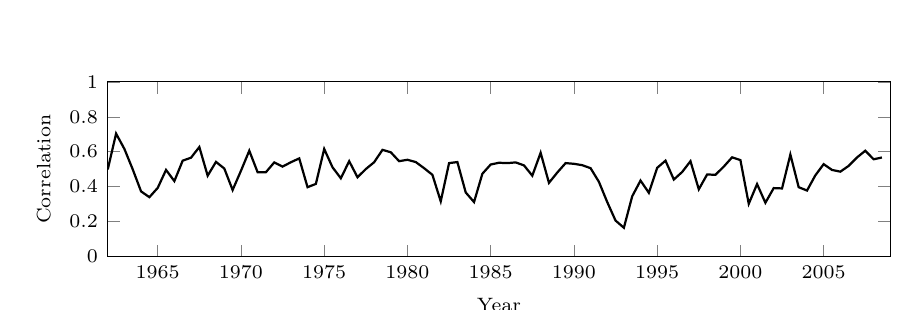
\begin{tikzpicture}
\begin{axis}[width=0.95\linewidth,height=3.8cm,xmin=1962,xmax=2009,ymin=0,ymax=1,
  xlabel={Year},ylabel={Correlation},
  tick label style={font=\scriptsize,/pgf/number format/1000 sep={}},label style={font=\scriptsize}]
\addplot[black,thick] coordinates {(1962.00,0.499) (1962.50,0.704) (1963.00,0.616) (1963.50,0.499) (1964.00,0.373) (1964.50,0.340) (1965.00,0.393) (1965.50,0.496) (1966.00,0.432) (1966.50,0.549) (1967.00,0.566) (1967.50,0.627) (1968.00,0.463) (1968.50,0.542) (1969.00,0.504) (1969.50,0.381) (1970.00,0.491) (1970.50,0.606) (1971.00,0.483) (1971.50,0.483) (1972.00,0.539) (1972.50,0.515) (1973.00,0.540) (1973.50,0.562) (1974.00,0.397) (1974.50,0.416) (1975.00,0.616) (1975.50,0.511) (1976.00,0.448) (1976.50,0.546) (1977.00,0.454) (1977.50,0.501) (1978.00,0.540) (1978.50,0.611) (1979.00,0.597) (1979.50,0.546) (1980.00,0.554) (1980.50,0.541) (1981.00,0.506) (1981.50,0.468) (1982.00,0.316) (1982.50,0.535) (1983.00,0.541) (1983.50,0.367) (1984.00,0.312) (1984.50,0.474) (1985.00,0.527) (1985.50,0.537) (1986.00,0.535) (1986.50,0.539) (1987.00,0.522) (1987.50,0.463) (1988.00,0.594) (1988.50,0.422) (1989.00,0.481) (1989.50,0.535) (1990.00,0.531) (1990.50,0.523) (1991.00,0.506) (1991.50,0.428) (1992.00,0.312) (1992.50,0.206) (1993.00,0.165) (1993.50,0.345) (1994.00,0.435) (1994.50,0.365) (1995.00,0.508) (1995.50,0.549) (1996.00,0.441) (1996.50,0.484) (1997.00,0.546) (1997.50,0.385) (1998.00,0.470) (1998.50,0.468) (1999.00,0.515) (1999.50,0.568) (2000.00,0.552) (2000.50,0.302) (2001.00,0.415) (2001.50,0.308) (2002.00,0.392) (2002.50,0.390) (2003.00,0.584) (2003.50,0.397) (2004.00,0.378) (2004.50,0.465) (2005.00,0.529) (2005.50,0.496) (2006.00,0.486) (2006.50,0.519) (2007.00,0.567) (2007.50,0.606) (2008.00,0.557) (2008.50,0.567)};
\end{axis}
\end{tikzpicture}
\end{center}
The conditional correlation ranges from 0.165 to 0.704 (mean 0.489); it dips sharply in 1992--93, when
IBM's own crisis made its returns idiosyncratic.
\intuicao{The DVEC treats each variance and covariance as a separate GARCH(1,1): simple and interpretable,
but with no volatility spillover between the two stocks and no built-in positive definiteness.}
\refbib{Tsay (2010) \S10.2.1 (Eq.~10.5, Example 10.2), pp.~510--513; \S8.1.4 (Eq.~8.7).}
\end{sol}

% ---------------------------------------------------------------- Q8 = T 10.3
\questao{BEKK(1,1) model for the S\&P index and HPQ (Tsay 10.3).}
\fonte{Tsay (2010), \textit{Analysis of Financial Time Series}, 3rd ed., Chapter~10, Exercise~10.3,
printed p.~554. Reproduced verbatim.}

\begin{quote}\small
10.3. Focus on the monthly log returns of the S\&P composite index and HPQ stock. Build a BEKK model for
the bivariate series. What is the fitted model? Plot the fitted volatility series and the time-varying
correlations.
\end{quote}
\resolespaco
\begin{sol}
\begin{notacao}
\item $\br_t=(r_{1t},r_{2t})'$: S\&P and HPQ log returns (\%), Jan 1962--Dec 2008, $T=564$; $\ba_t=\br_t-\bmu$.
\item $\bm C$: lower-triangular $2\times2$ (Tsay's $\bm A$); $\bm A_1,\bm B_1$: unrestricted $2\times2$ matrices.
\item $\otimes$: Kronecker product; covariance stationarity requires the eigenvalues of
$\bm A_1\otimes\bm A_1+\bm B_1\otimes\bm B_1$ to lie inside the unit circle.
\end{notacao}

\passo{model}{Tsay's Eq.~(10.6) with $m=s=1$ is
\begin{equation}
\bSigma_t=\bm C\bm C'+\bm A_1\ba_{t-1}\ba_{t-1}'\bm A_1'+\bm B_1\bSigma_{t-1}\bm B_1',\label{eq:q8bekk}
\end{equation}
positive definite whenever $\bm C\bm C'$ is positive semidefinite and $\bSigma_0$ is positive definite.
$(\bm A_1,\bm B_1)$ and $(-\bm A_1,-\bm B_1)$ give the same $\bSigma_t$; I normalise $A_{11,1},B_{11,1}>0$.
The likelihood is multimodal, so it is maximised from three starting points and the best maximum is kept.}

\passo{fitted model}{The 13-parameter maximum ($\ln L=-3536.57$) gives $\hat\mu_1=0.535_{(0.167)}$, $\hat\mu_2=1.128_{(0.389)}$, and
\begin{align}
\bSigma_t={}&\begin{pmatrix}1.160&0\\1.130&0.000\end{pmatrix}\begin{pmatrix}1.160&1.130\\0&0.000\end{pmatrix}
+\begin{pmatrix}0.427_{(0.060)}&-0.067_{(0.029)}\\0.586_{(0.155)}&0.022_{(0.075)}\end{pmatrix}\ba_{t-1}\ba_{t-1}'
\begin{pmatrix}0.427&0.586\\-0.067&0.022\end{pmatrix}\nonumber\\
&+\begin{pmatrix}0.847_{(0.030)}&0.038_{(0.011)}\\-0.311_{(0.076)}&1.037_{(0.015)}\end{pmatrix}\bSigma_{t-1}
\begin{pmatrix}0.847&-0.311\\0.038&1.037\end{pmatrix},\nonumber
\end{align}
so $\bm C\bm C'=\begin{pmatrix}1.345&1.311\\1.311&1.278\end{pmatrix}$ (standard errors of $\bm C$:
0.307, 0.940; the estimate $C_{22}$ sits on its boundary 0, where the Hessian standard error is not meaningful).
The spectral radius of $\hat{\bm A}_1\otimes\hat{\bm A}_1+\hat{\bm B}_1\otimes\hat{\bm B}_1$ is 0.9524,
below one, so the fitted process is covariance stationary even though $B_{22,1}=1.037>1$.}

\passo{interpretation}{Expanding \eqref{eq:q8bekk} element by element, HPQ's variance depends on
$(A_{21,1}a_{1,t-1}+A_{22,1}a_{2,t-1})^2$: the large, significant $A_{21,1}=0.586$ means market shocks
spill over into HPQ's volatility, while $A_{12,1}=-0.067$ makes the reverse spillover small. The
off-diagonal GARCH terms ($-0.311$, $0.038$) are significant too, so, unlike the DVEC of Q7, the two
volatilities are dynamically linked. Adequacy: $Q_2(5)=35.18$ ($p=0.019$), $Q_2(10)=48.62$ ($p=0.165$)
for the standardized residuals and $Q_2^{(2)}(5)=13.02$ ($p=0.876$), $Q_2^{(2)}(10)=32.83$ ($p=0.782$)
for their squares: the volatility dynamics are captured; a little low-order serial correlation remains
in the levels.}

\passo{plots}{Fitted volatilities and correlation (range 0.333--0.893, mean 0.607):}
\begin{center}
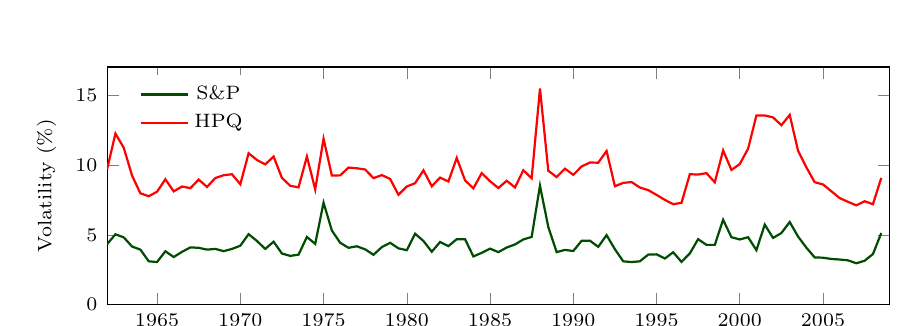
\begin{tikzpicture}
\begin{axis}[width=0.95\linewidth,height=4.6cm,xmin=1962,xmax=2009,ymin=0,
  ylabel={Volatility (\%)},legend pos=north west,legend style={font=\scriptsize,draw=none},
  tick label style={font=\scriptsize,/pgf/number format/1000 sep={}},label style={font=\scriptsize}]
\addplot[black!70!green,thick] coordinates {(1962.00,4.34) (1962.50,5.05) (1963.00,4.83) (1963.50,4.17) (1964.00,3.95) (1964.50,3.11) (1965.00,3.06) (1965.50,3.83) (1966.00,3.42) (1966.50,3.79) (1967.00,4.11) (1967.50,4.08) (1968.00,3.95) (1968.50,4.00) (1969.00,3.84) (1969.50,4.00) (1970.00,4.23) (1970.50,5.06) (1971.00,4.57) (1971.50,4.00) (1972.00,4.52) (1972.50,3.67) (1973.00,3.50) (1973.50,3.59) (1974.00,4.86) (1974.50,4.36) (1975.00,7.32) (1975.50,5.32) (1976.00,4.44) (1976.50,4.08) (1977.00,4.19) (1977.50,3.97) (1978.00,3.58) (1978.50,4.13) (1979.00,4.44) (1979.50,4.04) (1980.00,3.91) (1980.50,5.09) (1981.00,4.57) (1981.50,3.80) (1982.00,4.50) (1982.50,4.20) (1983.00,4.70) (1983.50,4.70) (1984.00,3.46) (1984.50,3.72) (1985.00,4.02) (1985.50,3.77) (1986.00,4.10) (1986.50,4.32) (1987.00,4.68) (1987.50,4.86) (1988.00,8.54) (1988.50,5.57) (1989.00,3.77) (1989.50,3.93) (1990.00,3.85) (1990.50,4.58) (1991.00,4.59) (1991.50,4.15) (1992.00,4.99) (1992.50,3.98) (1993.00,3.11) (1993.50,3.06) (1994.00,3.11) (1994.50,3.59) (1995.00,3.61) (1995.50,3.31) (1996.00,3.76) (1996.50,3.07) (1997.00,3.68) (1997.50,4.70) (1998.00,4.29) (1998.50,4.29) (1999.00,6.09) (1999.50,4.84) (2000.00,4.68) (2000.50,4.84) (2001.00,3.91) (2001.50,5.74) (2002.00,4.79) (2002.50,5.14) (2003.00,5.93) (2003.50,4.89) (2004.00,4.09) (2004.50,3.39) (2005.00,3.37) (2005.50,3.28) (2006.00,3.24) (2006.50,3.18) (2007.00,2.97) (2007.50,3.15) (2008.00,3.63) (2008.50,5.14)};
\addlegendentry{S\&P}
\addplot[red,thick] coordinates {(1962.00,9.72) (1962.50,12.28) (1963.00,11.26) (1963.50,9.26) (1964.00,7.99) (1964.50,7.78) (1965.00,8.11) (1965.50,9.00) (1966.00,8.13) (1966.50,8.48) (1967.00,8.36) (1967.50,8.98) (1968.00,8.45) (1968.50,9.09) (1969.00,9.29) (1969.50,9.36) (1970.00,8.64) (1970.50,10.87) (1971.00,10.38) (1971.50,10.07) (1972.00,10.63) (1972.50,9.10) (1973.00,8.53) (1973.50,8.42) (1974.00,10.63) (1974.50,8.27) (1975.00,11.91) (1975.50,9.27) (1976.00,9.28) (1976.50,9.84) (1977.00,9.79) (1977.50,9.70) (1978.00,9.08) (1978.50,9.30) (1979.00,9.02) (1979.50,7.89) (1980.00,8.48) (1980.50,8.72) (1981.00,9.64) (1981.50,8.50) (1982.00,9.12) (1982.50,8.84) (1983.00,10.53) (1983.50,8.92) (1984.00,8.35) (1984.50,9.44) (1985.00,8.86) (1985.50,8.37) (1986.00,8.89) (1986.50,8.41) (1987.00,9.65) (1987.50,9.07) (1988.00,15.51) (1988.50,9.61) (1989.00,9.16) (1989.50,9.76) (1990.00,9.32) (1990.50,9.92) (1991.00,10.20) (1991.50,10.19) (1992.00,11.03) (1992.50,8.50) (1993.00,8.74) (1993.50,8.80) (1994.00,8.41) (1994.50,8.22) (1995.00,7.88) (1995.50,7.52) (1996.00,7.21) (1996.50,7.31) (1997.00,9.36) (1997.50,9.34) (1998.00,9.44) (1998.50,8.78) (1999.00,11.07) (1999.50,9.67) (2000.00,10.09) (2000.50,11.19) (2001.00,13.58) (2001.50,13.58) (2002.00,13.44) (2002.50,12.88) (2003.00,13.62) (2003.50,11.05) (2004.00,9.85) (2004.50,8.79) (2005.00,8.63) (2005.50,8.14) (2006.00,7.65) (2006.50,7.38) (2007.00,7.13) (2007.50,7.42) (2008.00,7.21) (2008.50,9.10)};
\addlegendentry{HPQ}
\end{axis}
\end{tikzpicture}

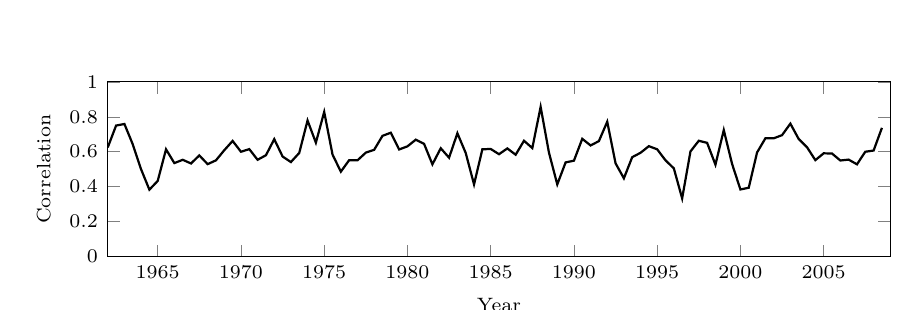
\begin{tikzpicture}
\begin{axis}[width=0.95\linewidth,height=3.8cm,xmin=1962,xmax=2009,ymin=0,ymax=1,
  xlabel={Year},ylabel={Correlation},
  tick label style={font=\scriptsize,/pgf/number format/1000 sep={}},label style={font=\scriptsize}]
\addplot[black,thick] coordinates {(1962.00,0.625) (1962.50,0.750) (1963.00,0.759) (1963.50,0.643) (1964.00,0.500) (1964.50,0.383) (1965.00,0.433) (1965.50,0.614) (1966.00,0.535) (1966.50,0.554) (1967.00,0.533) (1967.50,0.579) (1968.00,0.529) (1968.50,0.551) (1969.00,0.609) (1969.50,0.662) (1970.00,0.600) (1970.50,0.615) (1971.00,0.554) (1971.50,0.580) (1972.00,0.672) (1972.50,0.573) (1973.00,0.541) (1973.50,0.593) (1974.00,0.779) (1974.50,0.652) (1975.00,0.828) (1975.50,0.584) (1976.00,0.486) (1976.50,0.552) (1977.00,0.551) (1977.50,0.595) (1978.00,0.611) (1978.50,0.691) (1979.00,0.709) (1979.50,0.613) (1980.00,0.631) (1980.50,0.669) (1981.00,0.645) (1981.50,0.528) (1982.00,0.620) (1982.50,0.566) (1983.00,0.706) (1983.50,0.593) (1984.00,0.413) (1984.50,0.614) (1985.00,0.616) (1985.50,0.586) (1986.00,0.619) (1986.50,0.583) (1987.00,0.663) (1987.50,0.621) (1988.00,0.857) (1988.50,0.595) (1989.00,0.413) (1989.50,0.539) (1990.00,0.549) (1990.50,0.674) (1991.00,0.636) (1991.50,0.661) (1992.00,0.772) (1992.50,0.534) (1993.00,0.448) (1993.50,0.569) (1994.00,0.594) (1994.50,0.632) (1995.00,0.614) (1995.50,0.551) (1996.00,0.505) (1996.50,0.333) (1997.00,0.602) (1997.50,0.663) (1998.00,0.651) (1998.50,0.526) (1999.00,0.724) (1999.50,0.530) (2000.00,0.384) (2000.50,0.394) (2001.00,0.596) (2001.50,0.677) (2002.00,0.677) (2002.50,0.695) (2003.00,0.761) (2003.50,0.673) (2004.00,0.626) (2004.50,0.552) (2005.00,0.591) (2005.50,0.590) (2006.00,0.550) (2006.50,0.555) (2007.00,0.528) (2007.50,0.600) (2008.00,0.607) (2008.50,0.737)};
\end{axis}
\end{tikzpicture}
\end{center}
Correlations rise in market turmoil (1974--75, after the 1987 crash, 2002--03, late 2008): when the
market factor dominates, HPQ moves with it.
\intuicao{The quadratic form in \eqref{eq:q8bekk} buys positive definiteness and spillovers at the cost
of parameters with no direct meaning: only after multiplying out can one read the effect of each shock.}
\refbib{Tsay (2010) \S10.2.2 (Eq.~10.6, Example 10.3), pp.~513--516.}
\end{sol}

% ---------------------------------------------------------------- Q9 = T 10.4
\questao{Constant-correlation model for IBM, HPQ and the S\&P index (Tsay 10.4).}
\fonte{Tsay (2010), \textit{Analysis of Financial Time Series}, 3rd ed., Chapter~10, Exercise~10.4,
printed p.~554. Reproduced verbatim.}

\begin{quote}\small
10.4. Build a constant-correlation volatility model for the three monthly log returns of IBM stock, HPQ
stock, and S\&P composite index. Write down the fitted model. Is the model adequate? Why?
\end{quote}
\resolespaco
\begin{sol}
\begin{notacao}
\item $\br_t$: IBM, HPQ, S\&P log returns (\%), Jan 1962--Dec 2008, $T=564$; $\ba_t=\br_t-\bmu$.
\item $\sigma_{ii,t}$: conditional variance of $a_{it}$; $\alpha_{i0}>0$, $\alpha_{i1},\beta_{i1}\ge0$: its GARCH(1,1) parameters.
\item $\bm\rho=[\rho_{ij}]$: constant correlation matrix; $\bm D_t=\mathrm{diag}(\sigma_{11,t}^{1/2},\sigma_{22,t}^{1/2},\sigma_{33,t}^{1/2})$.
\end{notacao}

\passo{model}{Tsay's Eq.~(10.7) with a constant correlation matrix (Bollerslev, 1990), and a GARCH(1,1)
for each variance, is
\begin{align}
\bSigma_t&=\bm D_t\bm\rho\bm D_t,\label{eq:q9ccc}\\
\sigma_{ii,t}&=\alpha_{i0}+\alpha_{i1}a_{i,t-1}^2+\beta_{i1}\sigma_{ii,t-1},\qquad i=1,2,3.\label{eq:q9g}
\end{align}
With $\bm\epsilon_t=\bm D_t^{-1}\ba_t$, the log likelihood is
$-\tfrac12\sum_t[3\ln2\pi+\ln|\bm\rho|+2\sum_i\ln\sigma_{ii,t}^{1/2}+\bm\epsilon_t'\bm\rho^{-1}\bm\epsilon_t]$,
maximised jointly over 15 parameters.}

\passo{fitted model}{$\ln L=-5291.05$, $\hat\mu_1=0.783_{(0.275)}$, $\hat\mu_2=1.252_{(0.380)}$, $\hat\mu_3=0.530_{(0.172)}$, and
\begin{align}
\sigma_{11,t}&=1.472_{(1.043)}+0.057_{(0.022)}\,a_{1,t-1}^2+0.915_{(0.039)}\,\sigma_{11,t-1}\quad\text{(IBM)},\nonumber\\
\sigma_{22,t}&=4.424_{(2.049)}+0.061_{(0.018)}\,a_{2,t-1}^2+0.892_{(0.033)}\,\sigma_{22,t-1}\quad\text{(HPQ)},\nonumber\\
\sigma_{33,t}&=1.348_{(0.512)}+0.056_{(0.019)}\,a_{3,t-1}^2+0.873_{(0.032)}\,\sigma_{33,t-1}\quad\text{(S\&P)},\nonumber\\
\hat{\bm\rho}&=\begin{pmatrix}1&&\\0.494_{(0.032)}&1&\\0.605_{(0.028)}&0.623_{(0.026)}&1\end{pmatrix}.\nonumber
\end{align}
The three volatilities are persistent ($\alpha_{i1}+\beta_{i1}=0.972,\ 0.953,\ 0.929$) and the two stocks
correlate more with the index than with each other.}

\passo{adequacy}{Standardized residuals ($k=3$, so $9m$ d.f.):}
\begin{center}\small
\begin{tabular}{lrrrr}
\toprule
 & $Q_3(5)$ & $Q_3(10)$ & $Q_3^{(2)}(5)$ (squares) & $Q_3^{(2)}(10)$ (squares)\\
\midrule
Statistic & 54.51 & 82.01 & 53.86 & 93.85\\
$p$ value ($\chi^2_{45}$, $\chi^2_{90}$) & 0.156 & 0.714 & 0.171 & 0.370\\
\bottomrule
\end{tabular}
\end{center}
\textbf{Yes, by these checks the model is adequate}: no remaining serial or cross correlation in the
standardized residuals or their squares at 5\%. Why: the GARCH(1,1) equations absorb the volatility
clustering of each series, and with a constant $\bm\rho$ the standardized shocks behave like i.i.d.\
vectors. Caveat: the portmanteau tests do not test the constant-correlation restriction itself. The DVEC
fit of Q7 lets the IBM--HPQ correlation move between 0.17 and 0.70, and the BEKK of Q8 lets the
S\&P--HPQ correlation move between 0.33 and 0.89, which suggests that $\bm\rho$ is not constant; a
dynamic-correlation model (Q11) is the natural test.
\intuicao{The constant-correlation model reduces a $k$-dimensional volatility problem to $k$ univariate
GARCH models plus one correlation matrix: very parsimonious and always positive definite, but it rules
out the rise of correlations in crises that the other models detect.}
\refbib{Tsay (2010) \S10.3.1 (Eq.~10.7), \S10.4.1 (Eqs.~10.21--10.22, Examples 10.4--10.5), pp.~516--525.}
\end{sol}

% ---------------------------------------------------------------- Q10 = T 10.5
\questao{Constant-correlation GARCH for GE and the S\&P index, with a covariance forecast (Tsay 10.5).}
\fonte{Tsay (2010), \textit{Analysis of Financial Time Series}, 3rd ed., Chapter~10, Exercise~10.5,
printed p.~554. Reproduced verbatim.}

\begin{quote}\small
10.5. The file \texttt{m-geibmsp2608.txt} contains the monthly simple returns of General Electric stock,
IBM stock, and the S\&P composite index from January 1926 to December 2008. The returns include
dividends. Transform into log returns in percentages. Focus on the monthly log returns in percentages of
GE stock and the S\&P 500 index. Build a constant-correlation GARCH model for the bivariate series. Check
the adequacy of the fitted model, and obtain the 1-step-ahead forecast of the covariance matrix at the
forecast origin December 2008.
\end{quote}
\resolespaco
\begin{sol}
\begin{notacao}
\item $\br_t=(r_{1t},r_{2t})'$: GE and S\&P log returns (\%), Jan 1926--Dec 2008, $T=996$.
\item $\ba_t$: shocks of the mean equation; $\bm\sigma_t=(\sigma_{11,t},\sigma_{22,t})'$; $\ba_t^2=(a_{1t}^2,a_{2t}^2)'$; $\rho_{21}$: constant correlation.
\item $\bm\alpha_0$ ($2\times1$, positive), $\bm\alpha_1,\bm\beta_1$ ($2\times2$, nonnegative): volatility parameters;
$\bSigma_h(1)$: 1-step forecast of $\mathrm{Cov}(\ba_{h+1}\mid F_h)$ at origin $h=T$ (December 2008).
\end{notacao}

\passo{mean equation}{The returns are serially correlated: univariate $Q(12)=42.25$ (GE) and 34.58 (S\&P),
and the bivariate $Q_2(5)=64.51$ ($p=1.4\times10^{-6}$). A VAR(3) by OLS removes it (residual
$Q_2(5)=25.75$, $p=0.174$), so I use $\ba_t$ = VAR(3) residuals ($t=4,\dots,996$) and fit the volatility
model to them (two-step estimation; a constant $\bmu$ is kept in the volatility step).}

\passo{model}{Tsay's Eq.~(10.21)--(10.22), the bivariate constant-correlation GARCH(1,1), is
\begin{equation}
\bm\sigma_t=\bm\alpha_0+\bm\alpha_1\ba_{t-1}^2+\bm\beta_1\bm\sigma_{t-1},\qquad
\sigma_{21,t}=\rho_{21}(\sigma_{11,t}\sigma_{22,t})^{1/2},\label{eq:q10m}
\end{equation}
with the bivariate normal log density of Tsay's Eq.~(10.11). The diagonal version ($\bm\alpha_1,\bm\beta_1$
diagonal) has 9 parameters; the full version 13. Likelihood-ratio test:
\begin{align}
\mathrm{LR}&=2\left[(-5799.83)-(-5807.77)\right]\nonumber\\
&=15.90,\qquad \chi^2_4\ p=0.003,\nonumber
\end{align}
so the diagonal restriction is rejected: the volatilities interact.}

\passo{fitted model}{The full model (standard errors in parentheses; $\beta_{12,1}$ is on its bound 0, so it has
no standard error) gives $\hat\mu_1=0.339_{(0.199)}$, $\hat\mu_2=0.220_{(0.135)}$, and
\begin{align}
\begin{pmatrix}\sigma_{11,t}\\ \sigma_{22,t}\end{pmatrix}={}&
\begin{pmatrix}3.532_{(0.818)}\\0.315_{(0.696)}\end{pmatrix}
+\begin{pmatrix}0.098_{(0.021)}&0.028_{(0.033)}\\0.008_{(0.014)}&0.076_{(0.023)}\end{pmatrix}
\begin{pmatrix}a_{1,t-1}^2\\a_{2,t-1}^2\end{pmatrix}\nonumber\\
&+\begin{pmatrix}0.821_{(0.027)}&0.000\\0.063_{(0.056)}&0.767_{(0.084)}\end{pmatrix}
\begin{pmatrix}\sigma_{11,t-1}\\ \sigma_{22,t-1}\end{pmatrix},\nonumber\\
\hat\rho_{21}={}&0.780_{(0.013)}.\nonumber
\end{align}
The eigenvalues of $\hat{\bm\alpha}_1+\hat{\bm\beta}_1$ are 0.9392 and 0.8218, both positive and below 1, so
by Tsay's result 1 (p.~522) the shocks have a finite, positive-definite unconditional covariance matrix.
GE's variance responds mainly to its own past; the S\&P variance loads on GE's past variance
($0.063$), the coupling that the LR test detects. (The diagonal model, for comparison: GE
$\sigma_{11,t}=3.657+0.093a_{1,t-1}^2+0.835\sigma_{11,t-1}$, S\&P $\sigma_{22,t}=1.401+0.090a_{2,t-1}^2+0.852\sigma_{22,t-1}$,
$\hat\rho_{21}=0.781$.)}

\passo{adequacy}{Standardized residuals of the full model: $Q_2(5)=28.62$ ($p=0.095$), $Q_2(10)=45.45$
($p=0.255$); squares: $Q_2^{(2)}(5)=7.98$ ($p=0.992$), $Q_2^{(2)}(10)=21.76$ ($p=0.992$). Nothing rejects at
5\%: the model is adequate for the mean (after the VAR(3)) and for the volatility.}

\passo{forecast}{Shifting \eqref{eq:q10m} one period ahead, with $\ba_T$ and $\bm\sigma_T$ known at the origin
(Tsay p.~522, result 4):
\begin{equation}
\bm\sigma_T(1)=\bm\alpha_0+\bm\alpha_1\ba_T^2+\bm\beta_1\bm\sigma_T,\qquad \sigma_{21,T}(1)=\rho_{21}[\sigma_{11,T}(1)\sigma_{22,T}(1)]^{1/2}.\label{eq:q10f}
\end{equation}
At December 2008, $\ba_T=(-6.670,\ -0.005)'$, so $\ba_T^2=(44.489,\ 0.000)'$, and $\bm\sigma_T=(134.627,\ 60.177)'$.
The two products in \eqref{eq:q10f} are
\begin{align}
\hat{\bm\alpha}_1\ba_T^2&=\begin{pmatrix}0.0976(44.489)+0.0281(0.000)\\ 0.00762(44.489)+0.0758(0.000)\end{pmatrix}=\begin{pmatrix}4.342\\0.339\end{pmatrix},\nonumber\\
\hat{\bm\beta}_1\bm\sigma_T&=\begin{pmatrix}0.82104(134.627)+0(60.177)\\0.06334(134.627)+0.76651(60.177)\end{pmatrix}
=\begin{pmatrix}110.534\\8.527+46.126\end{pmatrix}=\begin{pmatrix}110.534\\54.654\end{pmatrix}.\nonumber
\end{align}
Substituting into \eqref{eq:q10f}:
\begin{align}
\sigma_{11,T}(1)&=(3.532)+(4.342)+(110.534)=118.41,\nonumber\\
\sigma_{22,T}(1)&=(0.315)+(0.339)+(54.654)=55.31,\nonumber\\
\sigma_{21,T}(1)&=(0.7800)\sqrt{(118.408)(55.308)}=(0.7800)(80.925)=63.12.\nonumber
\end{align}
Hence
\begin{equation}
\hat\bSigma_T(1)=\begin{pmatrix}118.41&63.12\\63.12&55.31\end{pmatrix},\nonumber
\end{equation}
i.e.\ forecast volatilities of 10.9\% (GE) and 7.4\% (S\&P) for January 2009, far above their
long-run levels after the late-2008 crisis. The diagonal model gives a similar picture
($110.31$, $46.91$, covariance $56.17$).}
\intuicao{A constant-correlation model forecasts the covariance only through the variances: it scales
up together with them in a crisis, but the correlation itself stays at 0.78.}
\refbib{Tsay (2010) \S10.4.1 (Eqs.~10.11, 10.21--10.22, Examples 10.4--10.5), pp.~516--525.}
\end{sol}

% ---------------------------------------------------------------- Q11 = T 10.6
\questao{Dynamic conditional correlation model for GE, IBM and the S\&P index (Tsay 10.6).}
\fonte{Tsay (2010), \textit{Analysis of Financial Time Series}, 3rd ed., Chapter~10, Exercise~10.6,
printed p.~554. Reproduced verbatim.}

\begin{quote}\small
10.6. Again, consider the monthly log returns of GE, IBM, and S\&P composite index from January 1926 to
December 2008. Build a dynamic correlation model for the three-dimensional series. For simplicity, use
the sample correlation matrix for $\bm\rho$ in Eq.~(10.32).
\end{quote}
\resolespaco
\begin{sol}
\begin{notacao}
\item $\br_t$: GE, IBM, S\&P log returns (\%), Jan 1926--Dec 2008; $\ba_t$: VAR(3) mean-equation shocks ($T=993$).
\item $\sigma_{ii,t}$: GARCH(1,1) variance of $a_{it}$; $\bm D_t=\mathrm{diag}(\sigma_{ii,t}^{1/2})$; $\bm\epsilon_t=\bm D_t^{-1}\ba_t$.
\item $\bm\rho_t$: conditional correlation matrix; $\hat{\bm\rho}$: sample correlation matrix of the returns;
$\bm\psi_{t-1}$: correlation matrix of $\bm\epsilon_{t-m},\dots,\bm\epsilon_{t-1}$, $m=4$; $\theta_1,\theta_2\ge0$, $\theta_1+\theta_2<1$.
\end{notacao}

\passo{model}{$\bSigma_t=\bm D_t\bm\rho_t\bm D_t$ (Tsay Eq.~10.7), each variance a GARCH(1,1) (Eq.~10.31 with
$\bm\Lambda_3=\bm0$, i.e.\ no leverage term), and the correlation equation Tsay's Eq.~(10.32):
\begin{equation}
\bm\rho_t=(1-\theta_1-\theta_2)\hat{\bm\rho}+\theta_1\bm\psi_{t-1}+\theta_2\bm\rho_{t-1},\qquad
\psi_{ij,t-1}=\frac{\sum_{h=1}^{m}\epsilon_{i,t-h}\epsilon_{j,t-h}}{\big(\sum_{h=1}^{m}\epsilon_{i,t-h}^2\sum_{h=1}^{m}\epsilon_{j,t-h}^2\big)^{1/2}}.\label{eq:q11dcc}
\end{equation}
$\bm\rho_t$ is a convex combination of correlation matrices, positive definite because $\hat{\bm\rho}$ is
and $1-\theta_1-\theta_2>0$; $m=4\geq k$ (Tse and Tsui's choice). As in Q10, a VAR(3) mean equation is used
(the returns have $Q_3(5)=107.97$; the VAR(3) residuals $45.72$, $p=0.442$). Estimation is two-step Gaussian
QMLE: (1) a univariate GARCH(1,1) for each $a_{it}$; (2) $(\theta_1,\theta_2)$ maximize the correlation part
$-\tfrac12\sum_t[\ln|\bm\rho_t|+\bm\epsilon_t'\bm\rho_t^{-1}\bm\epsilon_t]$.}

\passo{step 1: volatilities}{
\begin{align}
\sigma_{11,t}&=1.461+0.112\,a_{1,t-1}^2+0.866\,\sigma_{11,t-1}\quad\text{(GE)},\nonumber\\
\sigma_{22,t}&=3.242+0.105\,a_{2,t-1}^2+0.828\,\sigma_{22,t-1}\quad\text{(IBM)},\nonumber\\
\sigma_{33,t}&=0.608+0.127\,a_{3,t-1}^2+0.860\,\sigma_{33,t-1}\quad\text{(S\&P)},\nonumber
\end{align}
with means $0.273$, $0.129$, $0.205$ in the volatility step.}

\passo{step 2: correlations}{The sample correlations of the returns are $\hat\rho_{21}=0.556$ (GE--IBM),
$\hat\rho_{31}=0.828$ (GE--S\&P), $\hat\rho_{32}=0.645$ (IBM--S\&P). Maximizing gives
\begin{equation}
\hat\theta_1=0.0454\ (0.0080),\qquad \hat\theta_2=0.9228\ (0.0146),\label{eq:q11th}
\end{equation}
so the fitted correlation equation \eqref{eq:q11dcc} is
\begin{align}
\bm\rho_t&=(1-0.0454-0.9228)\hat{\bm\rho}+0.0454\,\bm\psi_{t-1}+0.9228\,\bm\rho_{t-1}\nonumber\\
&=0.0318\,\hat{\bm\rho}+0.0454\,\bm\psi_{t-1}+0.9228\,\bm\rho_{t-1}.\nonumber
\end{align}
Correlations are persistent ($\hat\theta_1+\hat\theta_2=0.9682$) but respond to recent co-movement. Against
constant correlations ($\theta_1=\theta_2=0$, $\bm\rho_t=\hat{\bm\rho}$) the likelihood ratio is 142.94; the
null puts $\theta_1$ on the boundary and leaves $\theta_2$ unidentified, so the $\chi^2_2$ reference is only
indicative, but the gain is overwhelming.}

\passo{adequacy and correlations}{Standardized residuals: $Q_3(5)=57.68$ ($p=0.097$), $Q_3(10)=97.58$
($p=0.275$); squares: $Q_3^{(2)}(5)=50.23$ ($p=0.274$), $Q_3^{(2)}(10)=86.70$ ($p=0.579$). The model is adequate.
The fitted correlations range over $[0.181,\ 0.751]$ (GE--IBM), $[0.465,\ 0.901]$ (GE--S\&P) and
$[0.335,\ 0.793]$ (IBM--S\&P): far from constant, which answers the caveat of Q9.}
\intuicao{The DCC idea is to separate the problem: univariate GARCH models take care of each volatility,
and two scalar parameters drive all correlations. Parsimony has a price, stressed by Tsay: every pair of
assets has the same correlation dynamics.}
\refbib{Tsay (2010) \S10.4.3 (Eqs.~10.31--10.32), pp.~531--536; \S10.3.1 (Eq.~10.7).}
\end{sol}

% =============================================================================
\bloco{4}{Bayesian SUR with serially correlated errors}{Greenberg Ch.~10 \,\textbullet\, Question 12}

% ---------------------------------------------------------------- Q12 = G 10.4
\questao{SUR model with first-order autocorrelation: a Gibbs algorithm (Greenberg 10.4).}
\fonte{Greenberg (2007), \textit{Introduction to Bayesian Econometrics}, 1st ed., Chapter~10
(Time Series), Section~10.6, Exercise~10.4, printed p.~167. Reproduced verbatim.}

\begin{quote}\small
10.4 Modify the SUR model to include first-order autocorrelation, and describe an algorithm for
estimating parameters.
\end{quote}
\resolespaco
\begin{sol}
\begin{notacao}
\item $j=1,\dots,J$: time periods; $s=1,\dots,S$: equations. $\bm y_j=(y_{1j},\dots,y_{Sj})'$; $\bm X_j$:
$S\times K$ block-diagonal covariate matrix of Greenberg's Eq.~(9.2); $\bm\beta$: $K\times1$ coefficients.
\item $\bm u_j$: $S\times1$ disturbances; $\bm R=\mathrm{diag}(\rho_1,\dots,\rho_S)$: AR(1) coefficients,
$|\rho_s|<1$; $\bm\rho=(\rho_1,\dots,\rho_S)'$; $\bm e_j\overset{iid}{\sim}N_S(\bm0,\bSigma)$: innovations.
\item Priors (Greenberg \S9.1 plus one block): $\bm\beta\sim N_K(\bm\beta_0,\bm B_0)$;
$\bSigma^{-1}\sim W_S(\nu_0,\bm R_0)$; $\bm\rho\sim N_S(\bm\rho_0,\bm P_0)\,\mathbf 1(\bm\rho\in\mathcal S)$,
$\mathcal S=(-1,1)^S$.
\item $\bm\Omega$: stationary covariance of $\bm u_j$; $g$: Gibbs iteration.
\end{notacao}

\passo{model}{Keep Greenberg's SUR Eq.~(9.2) and let each disturbance follow an AR(1):
\begin{align}
\bm y_j&=\bm X_j\bm\beta+\bm u_j,\label{eq:q12y}\\
\bm u_j&=\bm R\bm u_{j-1}+\bm e_j,\qquad \bm e_j\sim N_S(\bm0,\bSigma).\label{eq:q12u}
\end{align}
The innovations $\bm e_j$ are correlated across equations (the SUR feature) and independent over time;
the disturbances $\bm u_j$ are now correlated over time as well. (A fuller version replaces $\bm R$ by an
unrestricted $\bm\Phi$, a VAR(1) for $\bm u_j$; the algorithm below changes only in step (c).)}

\passo{quasi-differencing}{Premultiply \eqref{eq:q12y} at $j-1$ by $\bm R$ and subtract it from
\eqref{eq:q12y} at $j$; by \eqref{eq:q12u}, $\bm u_j-\bm R\bm u_{j-1}=\bm e_j$:
\begin{align}
\bm y_j-\bm R\bm y_{j-1}&=(\bm X_j-\bm R\bm X_{j-1})\bm\beta+(\bm u_j-\bm R\bm u_{j-1})\nonumber\\
\bm y_j^*&=\bm X_j^*\bm\beta+\bm e_j,\qquad j=2,\dots,J,\label{eq:q12star}
\end{align}
with $\bm y_j^*=\bm y_j-\bm R\bm y_{j-1}$ and $\bm X_j^*=\bm X_j-\bm R\bm X_{j-1}$. Given $\bm\rho$,
\eqref{eq:q12star} is an ordinary SUR model with serially independent errors. Conversely, given $\bm\beta$
the disturbances $\bm u_j=\bm y_j-\bm X_j\bm\beta$ are known, and \eqref{eq:q12u} can be written as a SUR
regression in $\bm\rho$:
\begin{equation}
\bm u_j=\bm U_{j-1}\bm\rho+\bm e_j,\qquad \bm U_{j-1}=\mathrm{diag}(u_{1,j-1},\dots,u_{S,j-1}).\label{eq:q12rho}
\end{equation}
This is the same two-way trick Greenberg uses for a single equation with AR($p$) errors in \S10.1.}

\passo{conditional posteriors}{Conditioning on $\bm y_1$ (likelihood of $j=2,\dots,J$), the full conditionals are:
\begin{enumerate}[label=(\alph*),leftmargin=2em]
\item $\bm\beta\mid\bm y,\bSigma,\bm\rho\sim N_K(\bar{\bm\beta},\bm B_1)$: Greenberg's Eq.~(9.4) applied to \eqref{eq:q12star},
\begin{equation}
\bm B_1=\Big(\sum_{j=2}^J\bm X_j^{*\prime}\bSigma^{-1}\bm X_j^*+\bm B_0^{-1}\Big)^{-1},\qquad
\bar{\bm\beta}=\bm B_1\Big(\sum_{j=2}^J\bm X_j^{*\prime}\bSigma^{-1}\bm y_j^*+\bm B_0^{-1}\bm\beta_0\Big).\label{eq:q12b}
\end{equation}
\item $\bSigma^{-1}\mid\bm y,\bm\beta,\bm\rho\sim W_S(\nu_1,\bm R_1)$: Greenberg's Eq.~(9.5) with the innovations
$\bm e_j=\bm y_j^*-\bm X_j^*\bm\beta$,
\begin{equation}
\nu_1=\nu_0+J-1,\qquad \bm R_1=\Big(\bm R_0^{-1}+\sum_{j=2}^J\bm e_j\bm e_j'\Big)^{-1}.\label{eq:q12w}
\end{equation}
\item $\bm\rho\mid\bm y,\bm\beta,\bSigma\sim N_S(\bar{\bm\rho},\bm P_1)\,\mathbf 1(\bm\rho\in\mathcal S)$: the same
normal-regression algebra applied to \eqref{eq:q12rho},
\begin{equation}
\bm P_1=\Big(\sum_{j=2}^J\bm U_{j-1}\bSigma^{-1}\bm U_{j-1}+\bm P_0^{-1}\Big)^{-1},\qquad
\bar{\bm\rho}=\bm P_1\Big(\sum_{j=2}^J\bm U_{j-1}\bSigma^{-1}\bm u_j+\bm P_0^{-1}\bm\rho_0\Big),\label{eq:q12r}
\end{equation}
drawn by rejection: draw from the normal until $|\rho_s|<1$ for all $s$.
\end{enumerate}
For an unrestricted $\bm\Phi$ in \eqref{eq:q12u}, write $\bm u_j=(\bm u_{j-1}'\otimes\bm I_S)\mathrm{vec}(\bm\Phi)+\bm e_j$
and use \eqref{eq:q12r} with $\bm U_{j-1}$ replaced by $\bm u_{j-1}'\otimes\bm I_S$, rejecting draws with an
eigenvalue of $\bm\Phi$ outside the unit circle.}

\passo{algorithm}{\textit{Algorithm (Gibbs sampler for SUR with AR(1) errors).}
\begin{enumerate}[label=\arabic*.,leftmargin=2em]
\item Choose $\bm\rho^{(0)}$ (e.g.\ $\bm0$) and $\bSigma^{-1(0)}$ (e.g.\ $\bm I_S$).
\item At iteration $g$: form $\bm y_j^*,\bm X_j^*$ with $\bm R^{(g-1)}$ and draw $\bm\beta^{(g)}$ from \eqref{eq:q12b}
with $\bSigma^{-1(g-1)}$.
\item Compute $\bm u_j=\bm y_j-\bm X_j\bm\beta^{(g)}$ and draw $\bm\rho^{(g)}$ from \eqref{eq:q12r} with $\bSigma^{-1(g-1)}$.
\item Compute $\bm e_j=\bm u_j-\bm R^{(g)}\bm u_{j-1}$ and draw $\bSigma^{-1(g)}$ from \eqref{eq:q12w}.
\item Repeat; discard a burn-in and use the remaining draws for posterior summaries.
\end{enumerate}}

\passo{first observation}{To use $\bm y_1$ exactly, note that stationarity of \eqref{eq:q12u} gives
$\bm u_1\sim N_S(\bm0,\bm\Omega)$ with $\bm\Omega=\bm R\bm\Omega\bm R'+\bSigma$, i.e.\
$\mathrm{vec}(\bm\Omega)=(\bm I_{S^2}-\bm R\otimes\bm R)^{-1}\mathrm{vec}(\bSigma)$ (the same algebra as Q3). Then
(i) in \eqref{eq:q12b} add $\bm X_1'\bm\Omega^{-1}\bm X_1$ to the precision and $\bm X_1'\bm\Omega^{-1}\bm y_1$ to
the mean term (still a Gibbs step); (ii) in steps 3 and 4 treat the draws above as proposals in a
Metropolis--Hastings step, accepted with probability
$\min\{1,\ N(\bm u_1\mid\bm0,\bm\Omega^{\mathrm{new}})/N(\bm u_1\mid\bm0,\bm\Omega^{\mathrm{old}})\}$, exactly as
Greenberg handles the initial $p$ observations of the AR($p$) model in \S10.1.}

\passo{numerical check}{The check script simulates $S=2$, $J=400$, each equation with an intercept and one
regressor, true $\bm\beta=(1,\ 0.5,\ -1,\ 2)'$, $\bm\rho=(0.6,\ -0.3)'$,
$\bSigma=\begin{pmatrix}1&0.5\\0.5&2\end{pmatrix}$, priors $\bm\beta\sim N(\bm0,100\bm I)$,
$\bm\rho\sim N(\bm0,\bm I)\mathbf 1(\mathcal S)$, $\bSigma^{-1}\sim W(4,\bm I)$, and runs 3000 iterations
(500 burn-in). Posterior means (standard deviations):
\begin{center}\small
\begin{tabular}{lrrrrrrrrr}
\toprule
 & $\beta_1$ & $\beta_2$ & $\beta_3$ & $\beta_4$ & $\rho_1$ & $\rho_2$ & $\sigma_{11}$ & $\sigma_{12}$ & $\sigma_{22}$\\
\midrule
Truth & 1 & 0.5 & $-1$ & 2 & 0.6 & $-0.3$ & 1 & 0.5 & 2\\
Mean & 1.156 & 0.589 & $-0.902$ & 2.106 & 0.561 & $-0.344$ & 0.869 & 0.473 & 1.835\\
s.d. & (0.107) & (0.039) & (0.051) & (0.061) & (0.038) & (0.044) & (0.061) & (0.068) & (0.132)\\
\bottomrule
\end{tabular}
\end{center}
Every posterior mean is within 3.5 posterior standard deviations of the truth (asserted in the script); the
gaps reflect sampling error of one simulated data set, not bias of the sampler.}
\intuicao{Autocorrelated disturbances make the data look like a regression only after quasi-differencing,
and quasi-differencing needs $\bm\rho$; Gibbs sampling breaks the circle by alternating: given $\bm\rho$,
estimate $\bm\beta$ by SUR-GLS on filtered data; given $\bm\beta$, estimate $\bm\rho$ by regressing residuals
on their lags; given both, update $\bSigma$ from the innovations.}
\refbib{Greenberg (2007) \S9.1 (Eqs.~9.1--9.5, Algorithm 9.1), pp.~134--137; \S10.1 (Eqs.~10.1--10.3), pp.~153--157.}
\end{sol}

\end{document}
